\section{HEATR}
\label{sHEATR}

\hypertarget{sHEATRhy}{The}
HEATR\index{HEATR|textbf} module generates pointwise heat production
\index{nuclear heating} cross sections and radiation damage
\index{radiation damage} energy production for specified reactions
and adds them to an existing PENDF\index{PENDF} file.  The heating
and damage numbers can then be easily group averaged, plotted, or
reformatted for other purposes.  An option of use to evaluators
checks ENDF/B files for neutron/photon energy-balance consistency.
\index{energy balance consistency}  The advantages of HEATR include

\begin{itemize}
\begin{singlespace}
\item Heating and damage are computed in a consistent way.

\item All ENDF/B neutron and photon data are used.

\item ENDF/B-6 charged-particle distributions are used
       when available.

\item Kinematic checks are available to improve future evaluations.

\item Both energy-balance and kinematic KERMA factors can be produced.
\end{singlespace}
\end{itemize}

This chapter describes the HEATR module in NJOY2016.0.

\subsection{Theory of Nuclear Heating}
\label{ssHEART_theory}

Heating is an important parameter of any nuclear system.  It may
represent the product being sold -- as in a power reactor -- or it may
affect the design of peripheral systems such as shields and structural
components.

Nuclear heating can be conveniently divided into neutron heating and
photon heating (see Fig.~\ref{f1}).  Neutron heating at a given
location is proportional to the local neutron flux and arises from the
kinetic energy of the charged products of a neutron induced reaction
(including both charged secondary particles and the recoil nucleus
itself).  Similarly, photon heating is proportional to the flux
of secondary photons transported from the site of previous neutron
reactions.  It is also traceable to the kinetic energy of charged
particles (for example, electron-positron pairs and recoil induced
by photoelectric capture).

\begin{figure}[thb]\centering
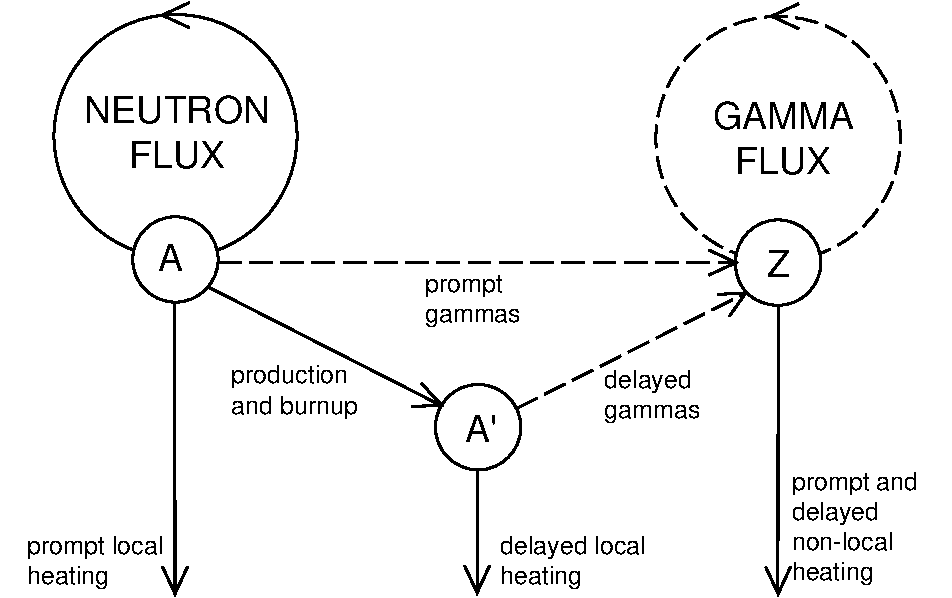
\includegraphics[height=3.4in, angle=0]{figs/heatr1}
\caption[Components of nuclear heating]{Components of nuclear
   heating.  HEATR treats the prompt
   local neutron heating only.  Gamma heating is computed
   in \hyperlink{sGAMINRhy}{GAMINR}.  Delayed local heating
   and photon production are
   not treated by NJOY, and they must be added at a later stage.}
\label{f1}
\end{figure}

Heating, therefore, is often described by
KERMA\cite{MACK}\index{KERMA} (Kinetic Energy Release in Materials)
coefficients $k_{ij}(E)$ defined such that the heating rate in a
mixture is given by

\begin{equation}
   H(E)=\sum_i\sum_j\rho_i k_{ij}(E)\phi(E)\,\,,
\label{HofE}
\end{equation}

\noindent
where $\rho_i$ is the number density of material $i$, $k_{ij}(E)$ is
the KERMA coefficient for material $i$ and reaction $j$ at incident
energy $E$, and $\phi(E)$ is the neutron or photon scalar flux at $E$.
KERMA is used just like a microscopic reaction cross section except
that its units are energy $\times$ cross section (eV-barns for HEATR).
When multiplied by a flux and number density, the result would give
heating in eV/s.

The ``direct method''\index{direct heating} for computing the KERMA
coefficient is

\begin{equation}
   k_{ij}(E)=\sum_\ell \overline{E}_{ij\ell}(E)\sigma_{ij}(E)\,\,,
\label{direct}
\end{equation}

\noindent
where the sum is carried out over all charged products of the reaction
including the recoil nucleus, and $\overline{E}_{ij\ell}$ is the total
kinetic energy carried away by the $\ell^{th}$ species of secondary
particle.  These kinds of data are now becoming available for some
materials with the advent of ENDF/B-VI and later, but earlier
ENDF/B versions did not include the detailed spectral information
needed to evaluate Eq.~\ref{direct}.

For this reason, NJOY computes KERMA factors for many materials by
the ``energy-balance method''\cite{Muir}.\index{energy-balance heating}
The energy allocated to neutrons and photons is simply subtracted
from the available energy to obtain the energy carried away by
charged particles:

\begin{equation}
   k_{ij}(E)=\Bigl(E+Q_{ij}-\overline{E}_{ijn}-\overline{E}_{ij\gamma}
      \Bigr)\,\sigma_{ij}(E)\,\,,
\label{kij}
\end{equation}
\vspace{0.5 pt}

\noindent
where $Q_{ij}$ is the mass-difference $Q$-value for material $i$ and
reaction $j$, $\overline{E}_n$ is the total energy of secondary
neutrons including multiplicity, and $\overline{E}_\gamma$ is the
energy of secondary photons including photon yields.

This method was well suited for use with ENDF/B-V\index{ENDF!ENDF/B-V},
or any other evaluation containing neutron and photon spectral
data, but not the
particle spectra required by the direct method.  The disadvantage
of this method is that the KERMA factor sometimes depends on a
difference between large numbers.  In order to obtain accurate
results, care must be taken by the evaluator to ensure
that photon and neutron yields and average energies are consistent.
In fact, the lack of consistency in ENDF/B-V often revealed itself
as negative KERMA\index{KERMA!negative KERMA} coefficients\cite{ebal}.

However, a negative KERMA coefficient is not always the defect it
seems to be.  It must be remembered that heating has both neutron and
photon components.  A negative KERMA might indicate that too much
energy has been included with the photon production in the evaluation.
This will result in excessive photon heating if most of the photons
stay in the system.  However, the negative KERMA will have just the
right magnitude to cancel this excess heating. The energy-balance
method guarantees conservation of total energy in large homogeneous
systems.

In this context, large and homogeneous means that most neutrons and
photons stay in their source regions.  It is clear that energy-balance
errors in the evaluation affect the spatial distribution of heat and
not the total system heating when the energy-balance method is
employed.

A final problem with the energy-balance method occurs for the
elemental evaluations\index{elemental heating} common in earlier
versions of ENDF/B.  Isotopic $Q$-values and cross sections
are not available in the files.  It will usually be possible to define
adequate cross sections, yields, and spectra for the element.  However,
it is clear that the available energy should be computed with an
effective Q given by

\begin{equation}
   \overline{Q}=\frac{\displaystyle\sum_i\rho_i\sigma_iQ_i}
      {\displaystyle\sum_i\rho_i\sigma_i}\,\,,
\end{equation}

\noindent
where $\rho_i$ is the atomic fraction of isotope $i$ in the element.
This number is energy dependent and can be represented only
approximately by the single constant Q allowed
in ENDF/B.  HEATR allows the user to input an auxiliary
energy-dependent Q for elements.\index{energy-dependent Q}

For elastic and discrete-level inelastic scattering, the neutron
KERMA coefficient can be evaluated directly without reference to
photon data.  For other reactions, conservation of momentum and
energy can be used to estimate the KERMA or to compute minimum and
maximum limits for the heating.  HEATR includes an option that tests
the energy-balance KERMA factors against these kinematic limits,
\index{kinematic heating tests} thereby providing a valuable test
of the neutron-photon consistency of the evaluation.  If the
energy-balance heating numbers for a particular isotope should
fail these tests, and if the isotope is important for a ``small''
system, an improved evaluation is probably required.  The
alternative of making {\it ad hoc} fixes to improve the local heat
production is dangerous because the faults in the neutron and/or photon
data revealed by the tests may lead to significant errors in neutron
transport and/or photon dose and nonlocal energy deposition.

In practice, an exception to this conclusion must be made for the
radiative capture reaction (n,$\gamma$).  The difference between the
available energy $E{+}Q$ and the total energy of the emitted photons is
such a small fraction of $E{+}Q$ that it is difficult to hold enough
precision to get reasonable recoil energies.  Moreover, the emitted
photons cause a component of recoil whose effect is not normally
included in evaluated capture spectra.  Finally, the ``element
problem'' cited above is especially troublesome for capture because
the available energy may change by several MeV between energies
dominated by resonances in different isotopes of the element, giving
rise to many negative or absurdly large heating numbers.  These
problems are more important for damage calculations (see below) where
the entire effect comes from recoil and the compensation provided by
later deposition of the photon energy is absent.

For these reasons, HEATR estimates the recoil due to radiative capture
\index{capture heating} using conservation of momentum.  The recoil
is the vector sum of the ``kick'' caused by the incident neutron
and the kicks due to the emission of all subsequent photons.  Assuming
that all photon emission is isotropic and that the directions of
photon emission are uncorrelated, the photon component of recoil
depends on the average of $E_\gamma^2$ over the entire photon spectrum

\begin{equation}
   E_R=\frac{E}{A+1}+\frac{\overline{E_\gamma^2}}{2(A+1)mc^2}\,\,,
\end{equation}
\vspace{0.5 pt}

\noindent
where $mc^2$ is the neutron mass energy.  The second term is important
below 25 -- 100 keV.  This formula gives an estimate that works for both
isotopes and elements and has no precision problems.  However, it
does not explicitly conserve energy, and isotopes with bad capture
photon data can still cause problems.

\subsection{Theory of Damage Energy}
\label{ssHEATR_damagetheory}

Damage to materials\index{radiation damage} caused by neutron
irradiation is an important design consideration in fission reactors
and is expected to be an even more important problem in fusion
power systems.  There are many radiation effects that may cause
damage, for example, direct heating, gas production ({\it e.g.},
helium embrittlement), and the production of lattice defects.

A large cluster of lattice defects can be produced by the primary
recoil nucleus of a nuclear reaction as it slows down in a lattice.
It has been shown that there is an empirical correlation between the
number of displaced atoms (DPA\index{DPA}, displacements per atom)
and various properties of metals, such as elasticity.  The number
of displaced atoms depends on the total available energy $E_a$ and
the energy required to displace an atom from its lattice position
$E_d$.  Since the available energy is used up by producing pairs,

\begin{equation}
   {\rm DPA}=\frac{E_a}{2E_d}\,\,.
\end{equation}
\vspace{0.5 pt}

\noindent
The values of $E_d$ used in practice are chosen to represent the
empirical correlations, and a wide range of values is found in the
literature\cite{Gabriel,Doran,Greenwood}.  Table~\ref{ade} gives
the default values used in NJOY2016.  The energy available to cause
displacements is what HEATR calculates.  It depends on the recoil
spectrum and the partition of recoil energy between electronic
excitations and atomic motion.  The partition function used is
given by Robinson\cite{Robinson} based on the electronic screening
theory of Lindhard\cite{Lindhard} (see Fig.~\ref{f2}).

\begin{table}[t]
\caption[Atomic Displacement Energy Data for DPA]{Typical
  Values for the Atomic Displacement Energy
  Needed to Compute DPA\cite{Greenwood}.}

\begin{center}
\begin{tabular}{cccc}
Element & $E_d$, eV & Element & $E_d$, eV \\ \hline
Be & 31 & Co & 40 \\
C  & 31 & Ni & 40 \\
Mg & 25 & Cu & 40 \\
Al & 27 & Zr & 40 \\
Si & 25 & Nb & 40 \\
Ca & 40 & Mo & 60 \\
Ti & 40 & Ag & 60 \\
V  & 40 & Ta & 90 \\
Cr & 40 & W  & 90 \\
Mn & 40 & Au & 30 \\
Fe & 40 & Pb & 25 \\ \hline
\end{tabular}
\end{center}
\label{ade}
\end{table}

\begin{figure}[t]\centering
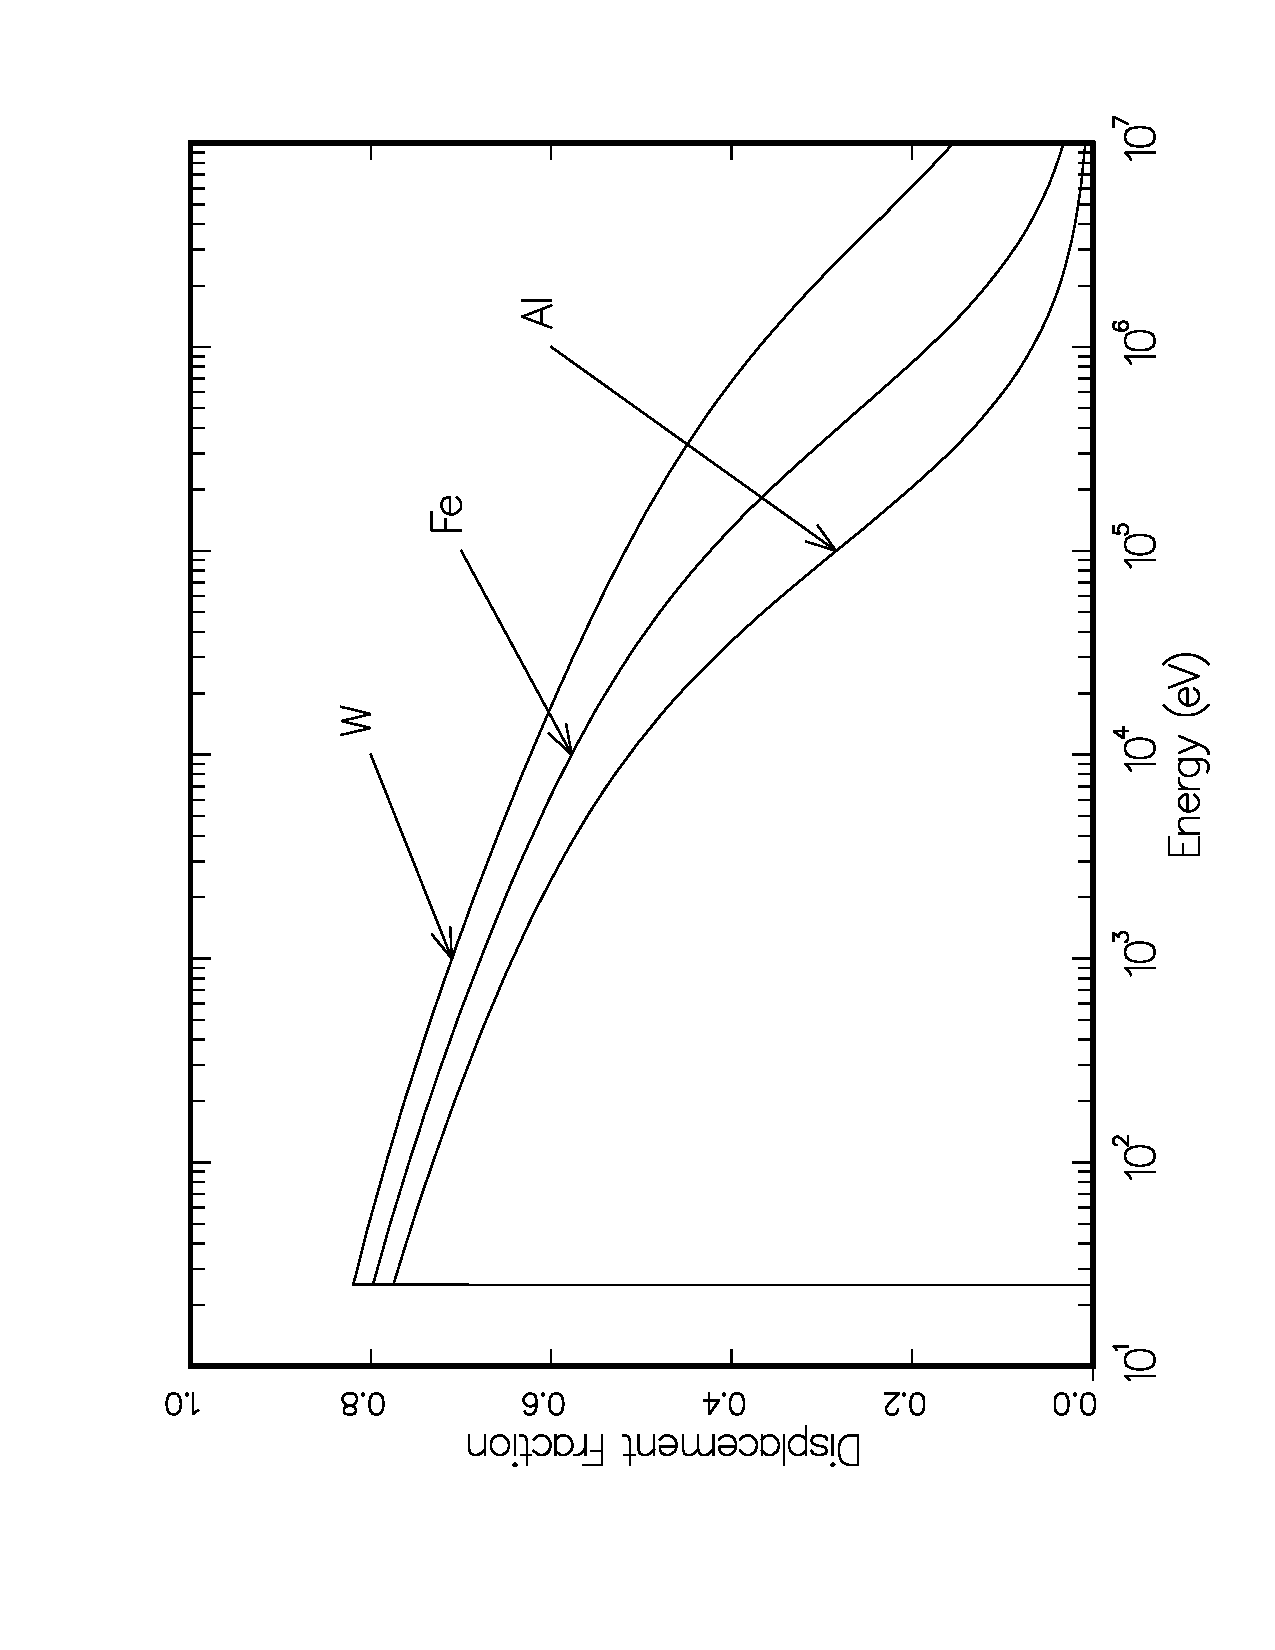
\includegraphics[height=4.0in, angle=270]{figs/heatr2ack}
\caption[Sample recoil energy and lattice displacement data]
  {Examples of the portion of the primary recoil
  energy that is available to cause lattice displacements in
  metallic lattices.  The remaining energy leads to electronic
  excitation.  The quantity plotted is $P(E)$ from
  Eq.~\ref{robinson} divided by $E$.  The 25 eV cutoff
  is also discussed in connection with Eq.~\ref{robinson}.}
\label{f2}
\end{figure}

The damage output from HEATR is the damage energy production
cross section (eV-barns).  As in Eq.~\ref{HofE}, multiplying by
the density and flux gives eV/s.  Dividing by $2E_d$ gives
displacements/s.  This result is often reduced by an efficiency
factor (say 80\%) to improve the fit to the empirical correlations.
\index{damage energy production}


\subsection{Computation of KERMA Factors By Energy Balance}
\label{ssHEATR_KERMA}

\subsubsection{The general case}
\label{sssHEATR_generalKERMA}

The older ENDF/B files do not usually give photon production data for
all partial reactions.  Summation reactions such as nonelastic
(MT=3) and inelastic (MT=4) are often used.  It is still possible
to compute partial KERMA factors for those summation reactions by
reordering Eq.~\ref{kij} as follows:

\begin{equation}
   k_{ij}=\sum_{j\in J}k_{ij}^n(E)-\sum_{\ell\in J}
    \overline{E}_{i\ell\gamma}\sigma_{i\ell}(E)\,\,,
\label{reordered}
\end{equation}
\vspace{0.5 pt}

\noindent
where $j$ runs over all neutron partials contained in $J$, and
$\ell$ runs over all photon partials in $J$.  The total KERMA is
well defined, but partial KERMAS should be used only with caution.

HEATR loops through all the neutron reactions on the ENDF/B tape.
If energy balance is to be used, it computes the neutron
contributions needed for the first term.  These are

\begin{equation}
   k_{ij}^n(E)=
    \Bigl[E+Q_{ij}-\overline{E}_{ijn}(E)\Bigr]\sigma_{ij}(E)\,\,.
\label{nkerm}
\end{equation}
\vspace{0.5 pt}

The $Q$-value is zero for elastic and inelastic scattering.  For
(n,n$'$) particle reactions represented by scattering with an
LR flag set, Q is the ENDF ``C1'' field from MF=3.  For most
other reactions, Q is the ``C2'' field from MF=3.  HEATR allows
users to override any $Q$-value with their own numbers.

The $\overline{E}_n$ value as used in Eq.~\ref{nkerm} is
defined to include multiplicity.  The multiplicity is either
implicit --- for example, 2 for (n,2n) --- or is retrieved from the
ENDF/B file (e.g. for the mt5 reaction).  The average energy per
neutron is computed differently for discrete two-body reactions
and continuum reactions.

For elastic and discrete inelastic scattering (MT=2, 51-90),

\begin{equation}
   \overline{E}_n=\frac{E}{(A+1)^2}\Bigl(1+2Rf_1+R^2\Bigr)\,\,,
\label{enb}
\end{equation}

\noindent
where $f_1$ is the center-of-mass (CM) average scattering cosine
from MF=4 and $R$ is the effective mass ratio.  For elastic
scattering, $R{=}A$, but for threshold scattering,

\begin{equation}
   R=A\sqrt{1-\frac{(A+1)S}{AE}}\,\,,
\end{equation}

\noindent
where $S$ is the negative of the C2 field from MF=3.

For continuum scattering, the average energy per neutron is
computed from the secondary neutron spectrum, $g$, in MF=5 using

\begin{equation}
   \overline{E}_n(E)=\int_0^U E'g(E,E')\,dE'\,\,,
\end{equation}

\noindent
where $U$ is defined in MF=5.  If $g$ is tabulated (LAW=1 or
LAW=5), the integral is carried out analytically for each panel
by making use of the ENDF/B interpolation laws.  For the simple
analytic representations (LAW=7, 9, or 11), the average energies
are known\cite{ENDF102}.

The neutron cross sections required by Eq.~\ref{nkerm} are
obtained from an existing PENDF\index{PENDF} file (see
\hyperlink{sRECONRhy}{RECONR}\index{RECONR},
and \hyperlink{sBROADRhy}{BROADR})\index{BROADR}.

When the neutron sum in Eq.~\ref{reordered} is complete, the
code processes the photon production files.  If the evaluation
does not include photon data, HEATR returns only the first sum.
This is equivalent to assuming that all photon energy is
deposited locally, consistent with the fact that there will
be no contribution to the photon transport source from this
material.  The same result can be forced by using the
\cword{local} parameter (see ``User Input'', Section~\ref{ssHEATR_inp}, below).

Discrete photon yields and energies are obtained from
MF=12 or 13.  Continuum photon data are obtained from MF=15,
and the average photon energy and $\overline{E_\gamma^2}$ are
computed.  For radiative capture, the photon term becomes

\begin{equation}
   E_\gamma\sigma_\gamma=\left(E+Q-\frac{E}{A+1}
    +\frac{\overline{E_\gamma^2}}{2(A+1)mc^2}\,Y_\gamma\right)
    \sigma_\gamma\,\,,
\label{cfix}
\end{equation}

\noindent
\cite{ENDF102}
where $Y_\gamma$ is the capture photon yield from MF=12.  This
corrects the capture contribution from Eq.~\ref{nkerm} by
conservation of momentum.  For other reactions,
Eq.~\ref{nkerm} is sufficient, and the product of
$\overline{E}_\gamma$, $Y_\gamma$, and $\sigma_\gamma$ is
subtracted from the neutron contribution.

\subsubsection{The special case of fission}
\label{sssHEATR_fissionKERMA}

The partial KERMA for fission is a special case due to the particular
problems with obtaining the $Q$-value for fission\index{fission Q}.
First, the fission $Q$-value given in the C1 field of MF=3 includes
delayed neutron and gamma contributions that we need to exclude,
and second, the $Q$-value for fission is energy dependent.

As a result, the KERMA for fission will be calculated differently
when compared to the other reactions which use Eq.~\ref{nkerm} as is.
Theoretically speaking, there is no difference with Eq.~\ref{nkerm}
as we will show here.

Energy dependent fission energy release and its components are given
in the MT=458 section of MF=1 on the ENDF file. This section of the
ENDF file defines the following components to the fission energy release:
\begin{itemize}
\item $Q_k$ : the kinetic energy of the fission fragments
\item $Q_{n,p}$ and $Q_{n,d}$ : the kinetic energy of the prompt and
      delayed fission neutrons
\item $Q_{\gamma,p}$ and $Q_{\gamma,d}$ : the energy of the prompt
      and delayed gamma rays
\item $Q_{\beta}$ : the energy of the delayed beta radiation
\item $Q_{\nu}$ : the energy carried away by the neutrinos
\end{itemize}

With these components, we can now define the total energy release
from fission $Q_t$, the total energy release from fission excluding
neutrinos $Q_r$ and the total prompt energy release from fission
$Q_p$ as as follows:
\begin{equation}
   Q_t(E) = Q_k(E) + Q_{n,p} + Q_{n,d} + Q_{\gamma,p} + Q_{\gamma,d}
          + Q_{\beta} + Q_{\nu}\,\,,
\end{equation}
\begin{equation}
   Q_r(E) = Q_t(E) - Q_{\nu}\,\,,
\end{equation}
\begin{equation}
   Q_p(E) = Q_r(E) - Q_{n,d} - Q_{\gamma,d} - Q_{\beta}
          = Q_k(E) + Q_{n,p} + Q_{\gamma,p}\,\,.
\end{equation}

Using these fission energy release components, we can define the
fission reaction $Q$-value (i.e. the energy released through the fission
reaction) as the prompt fission energy release minus the incident
neutron energy:
\begin{equation}
   Q(E) = Q_p(E) - E
        = Q_k(E) + Q_{n,p} + Q_{\gamma,p} - E\,\,.
\end{equation}

It should be noted that we have chosen to ignore the energy dependence
of delayed beta and gamma emission because we don't yet treat it in
subsequent codes. However, the impact of such an approximation is somewhat
limited due to the amount of energy involved. For example, for U235 the
value of $Q_k$ is roughly 169 MeV at 1e-5 eV while the sum of $Q_{n,d}$,
$Q_{\gamma,d}$ and $Q_{\beta}$ is roughly 12 MeV at 1e-5 eV.

For the calculation of the fission KERMA factor, we also need to know the
energy of the outgoing neutrons (i.e. $\overline{E}$ from Eq.~\ref{nkerm}).
Because we are considering the prompt energy release only, this is simply
equal to the prompt neutron energy release $Q_{n,p}$.

As a result, the partial fission KERMA factor $k_{f}^n$ will be given by:
\begin{equation}
   k_{f}^n(E)=
    \Bigl[E + Q(E) - \overline{E}(E)\Bigr]\sigma_{f}(E)
             =
    \Bigl[Q_k(E) + Q_{\gamma,p}(E)\Bigr]\sigma_{f}(E)\,\,.
\label{fkerm}
\end{equation}

The fission KERMA is thus equal to the fission cross section times the
sum of the kinetic energy of the fission products and the prompt gamma
energy release. This value will then be used in Eq.~\ref{reordered} to
calculate the total KERMA.

In some cases it is possible that a fissile nuclide does not have an
MT458 section. In this case, Eq.~\ref{nkerm} will be used directly as
follows:
\begin{equation}
   k_{f}^n(E)=
    \Bigl[E + Q(E) - \overline{\nu}(E)\overline{E}(E)\Bigr]\sigma_{f}(E)
\label{fkerm-nomt458}
\end{equation}
where the fission $Q$-value is approximated using the thermal point
energy dependencies defined for MT458:
\begin{equation}
   Q(E) = Q_{\text{ENDF}} - 8070000 \left(\overline{\nu}(E)-\overline{\nu}(0)\right) + 0.307 E
\end{equation}

In this equation, $Q_{\text{ENDF}}$ is the reaction $Q$-value for fission
as given in MF3.

\subsection{Kinematic Limits}
\label{ssHEATR_kinematiclimits}

As an option provided  mainly as an aid to evaluators, HEATR
will compute the kinematic maximum and minimum KERMA
\index{kinematic limits} coefficients and compare them with the
energy-balance results.  The formulas are as follows.  For
elastic scattering (MT=2), the expected recoil energy is

\begin{equation}
   \overline{E}_R=\frac{2AE}{(A+1)^2}(1-f_1)\,\,.
\end{equation}

For discrete-inelastic scattering (MT=51-90), the photon
momentum is neglected to obtain

\begin{equation}
   \overline{E}_R=\frac{2AE}{(A+1)^2}\left[\,1-
    f_1\sqrt{1-\frac{(A+1)E_\gamma}{AE}}\,\,\right]
    -\frac{E_\gamma}{A+1}\,\,,
\label{disc}
\end{equation}

\noindent
where $E_\gamma{=}-$C2 from MF=3.  For continuum inelastic
scattering (MT=91), secondary neutrons are assumed to be
isotropic in the laboratory system (LAB) giving

\begin{equation}
   \overline{E}_R=\frac{E-E_n}{A}\,\,,
\label{contin}
\end{equation}

\noindent
and

\begin{equation}
   \overline{E}_\gamma=
     \frac{(A-1)E-(A+1)\overline{E}_n}{A}\,\,,
\label{contin2}
\end{equation}
\vspace{0.5 pt}

\noindent
where $\overline{E}_\gamma$ is the average photon energy
expected for this representation.  For radiative capture (MT=102),

\begin{equation}
   \overline{E}_R=\frac{E}{A+1}+E_K
\end{equation}

\noindent
and

\begin{equation}
   \overline{E}_\gamma=Q+\frac{AE}{A+1}-E_K\,\,,
\end{equation}

\noindent
where

\begin{equation}
   E_K=\frac{1}{2M_Rc^2}\left[\frac{AE}{A+1}+Q\right]^2
     \left\{1-\frac{1}{M_Rc^2}\left[
       \frac{AE}{A+1}+Q\right]\right\}\,\,,
\end{equation}

\noindent
with

\noindent
\begin{equation}
   M_Rc^2=(939.565\times 10^6)(A+1)-Q
\end{equation}

\noindent
being the mass energy in eV.  The value of this constant is
actually computed from fundamental constants in NJOY2016.

For two-body scattering followed by particle emission
(MT=51-91, LR flag set), a minimum and maximum can be defined:

\begin{eqnarray}
   (E'_R+E_x)_{\rm min}&=&\overline{E}_R\,\,,\;\hbox{and}\\
   (E'_R+E_x)_{\rm max}&=&\overline{E}_R+Q+(E_\gamma)_{\rm max}\,\,,
\end{eqnarray}

\noindent
where $\overline{E}_R$ is the value from Eq.~\ref{disc} or
(\ref{contin}), $Q$ is the C2 field from File 3, and
$(E_\gamma)_{\rm max}$ is the negative of the C2 field from
File 3.  In these equations, $E'_R$ is the recoil energy
and $E_x$ is the energy of the charged product.  For
absorption followed by particle emission (MT=103-120),

\begin{eqnarray}
   (E_R+E_x)_{\rm min}&=&\frac{E}{A+1-x}\,\,,\\
   (E_\gamma)_{\rm max}&=&Q+\frac{A-x}{A+1-x}\,E\,\,,\;\hbox{and}\\
   (E_R+E_x)_{\rm max}&=&E+Q\,\,,
\end{eqnarray}

\noindent
where $Q$ is the C2 field from MF=3 and $x$ is the particle mass
ratio ($x{=}1$ gives a minimum for all reactions).
For (n,2n) reactions,

\begin{eqnarray}
   (E_R)_{\rm min}&=&0\,\,,\;\hbox{and}\\
   (E_R)_{\rm max}&=&\frac{E+\overline{E}_n}{A-1}\,\,,
\end{eqnarray}

\noindent
and for (n,3n) reactions,

\begin{eqnarray}
   (E_R)_{\rm min}&=&0\,\,,\;\hbox{and}\\
   (E_R)_{\rm max}&=&\frac{E+2\overline{E}_n}{A-2}\,\,.
\end{eqnarray}

\noindent
For both (n,2n) and (n,3n), if $(E_R)_{\rm max}$ is greater than
$E_R$, it is set equal to $E_R$.  In addition, these formulas
are not used for $A{<}10$; $(E_R)_{\rm max}$ is set to $E_R$.
For other neutron continuum scattering reactions (MT=22-45),

\begin{eqnarray}
   (E_R+E_x)_{\rm min}&=&0\,\,,\;\hbox{and}\\
   (E_R+E_x)_{\rm max}&=&E+Q-\overline{E}_n\,\,,
\end{eqnarray}

\noindent
where $Q$ is the C2 field from File 3.  Finally, for fission
(MT=18-21, 38), the limits are

\begin{eqnarray}
   (E_R)_{\rm min}&=&E+Q-\frac{1}{2}
    \overline{E}_n-15{\times}10^6\,\hbox{\rm eV}\,\,,\;\hbox{and}\\
   (E_R)_{\rm max}&=&E+Q-\overline{E}_n\,\,,
\end{eqnarray}

\noindent
where $Q$ is the prompt fission Q-value less neutrinos.  It
is determined by taking the total (less neutrinos) value from
File 3 and subtracting the delayed energy obtained from
MF=1/MT=458.

These values are intended to be very conservative.  Note
that $E_K$ is only significant at very low neutron energy.
In order to reduce unimportant error messages, a tolerance
band is applied to the above limits.  If all checks are
satisfied, the resulting KERMA coefficients should give good
local heating results even when 99.8\% of the photons
escape the local region.  More information on using the
kinematic checks to diagnose energy-balance problems in
evaluations will be found in ``Diagnosing Energy-Balance
Problems'', Section~\ref{ssHEATR_EB_Prob}.\index{energy balance consistency}

The upper kinematic limit can also be written out to the
output tape as MT=443 if desired.  It is similar to the KERMA
factors generated by the MACK code\cite{MACK}, and it is
sometimes preferable to the energy-balance KERMA for
calculating local heating for evaluations with severe
energy-balance problems.  The kinematic value in MT=443
is useful for plots (see the examples in this report).

\subsection{Computation of Damage Energy}
\label{ssHEATR_damagecomputation}

The formulas used for calculating damage energy are derived
\index{damage energy production}
from the same sources as the heating formulas given above,
except in this case, the effects of scattering angle do not
result in simple factors like $f_1$ because the Robinson
partition function is not linear.  Instead, it is
\index{Robinson partition function}
calculated as follows:

\begin{equation}
   P(E)=\frac{E_R}{1+F_L(3.4008\epsilon^{1/6}+0.40244\epsilon^{3/4}
     +\epsilon)}\,\,,
\label{robinson}
\end{equation}
\vspace{0.5 pt}

\noindent
if $E_R\ge 25.0$ eV, and zero otherwise.  In Eq.~\ref{robinson},
$E_R$ is the primary recoil energy,

\begin{eqnarray}
   \epsilon&=&\frac{E_R}{E_L}\,\,,\\
   E_L&=&30.724Z_RZ_L\left(Z_R^{2/3}+Z_L^{2/3}\right)^{1/2}
     (A_R+A_L)/A_L\,\,,\;\hbox{and}\\
   F_L&=&\frac{0.0793Z_R^{2/3}Z_L^{1/2}\left(A_R+A_L\right)^{3/2}}
      {\left(Z_R^{2/3}+Z_L^{2/3}\right)^{3/4}A_R^{3/2}A_L^{1/2}}\,\,,
\end{eqnarray}

\noindent
and $Z_i$ and $A_i$ refer to the charge and atomic number
of the lattice nuclei (L) and the recoil nuclei (R).  The
function behaves like $E_R$ at low recoil energies and then
levels out at higher energies.  Therefore, the damage-energy
production cross section is always less than the heat
production cross section.  See Fig.~\ref{f2} for examples.

For elastic and two-body discrete-level inelastic scattering,

\begin{equation}
   E_R(E,\mu)=\frac{AE}{(A+1)^2}\Bigl(1-2R\mu+R^2\Bigr)\,\,,
\label{tworec}
\end{equation}
\vspace{0.5 pt}

\noindent
where the ``effective mass'' is given by

\begin{equation}
   R=\sqrt{1-\frac{(A+1)(-Q)}{AE}}\,\,,
\end{equation}

\noindent
and $\mu$ is the CM scattering cosine.  The damage energy
production cross section is then obtained from

\begin{equation}
   D(E)=\sigma(E)\int_{-1}^1 f(E,\mu)\,
     P(E_R[E,\mu])\,d\mu\,\,,
\label{damint}
\end{equation}

\noindent
where $f$ is the angular distribution from the ENDF/B File 4.
This integration is performed with a 20-point Gauss-Legendre
quadrature.  Discrete-level reactions with LR flags to
indicate, for example, (n,n$'$)$\alpha$ reactions, are
treated in the same way at present.  The additional emitted
particles are ignored.

Continuum reactions like (n,n$'$) give a recoil spectrum

\begin{equation}
   E_R(E,E',\mu)=\frac{1}{A}\Bigl(E-2\sqrt{EE'}\mu+E'\Bigr)\,\,,
\end{equation}

\noindent
where $E'$ is the secondary neutron energy, $\mu$ is the
laboratory cosine, and the photon momentum has been neglected.
The damage becomes

\begin{equation}
   D(E)=\sigma(E)\int_0^\infty\,dE'\,\int_{-1}^1d\mu
     \, f(E,\mu)\,g(E,E')\,P(E_R[E,E',\mu])\,\,,
\label{f5dam}
\end{equation}

\noindent
where $g$ is the secondary energy distribution from File 5.
In the code, the angular distribution is defaulted to isotropic,
and a 4-point Gaussian quadrature is used for the angular
integration.  For analytic representations of $g$, an adaptive
integration to 5\% accuracy is used for $E'$; for tabulated
File 5 data, a trapezoidal integration is performed using the
energy grid of the file.  The same procedure is used for
(n,2n), (n,3n), etc., but it is not realistic for reactions
like (n,n$'$p) or (n,n$'\alpha$).  The neutron in these types of
reactions can get out of the nucleus quite easily; thus, much of
the energy available to secondary particles is typically carried
away by the charged particles\cite{alb}.  HEATR treats these
reactions in the same way as (n,p) or (n,$\alpha$).

The recoil for radiative capture must include the momentum of
the emitted photons below 25 -- 100 keV giving

\begin{equation}
   E_R=\frac{E}{A+1}-2\sqrt{\frac{E}{A+1}}
    \sqrt{\frac{E_\gamma^2}{2(A+1)mc^2}}\cos\phi
    +\frac{\overline{E_\gamma^2}}{2(A+1)mc^2}\,\,,
\label{radrec}
\end{equation}

\noindent
where $\phi$ is the angle between the incident neutron direction
and emitted photon direction.  If subsequent photons are emitted
in a cascade, each one will add an additional term of
$\overline{E_\gamma^2}$ and an additional angle.  A complete
averaging of Eq.~\ref{radrec} with respect to $P(E_R)$ would
be very difficult and would require angular correlations not
present in ENDF/B evaluations.  However, damage calculations are still
fairly crude, and an estimate for the damage obtained by
treating the neutron ``kick'' and all the photon kicks
independently should give a reasonable upper limit because

\begin{equation}
   \int_{-1}^1D(E_R)\,d\cos\phi\le
     D\left(\frac{E}{A+1}\right)+\sum_\gamma D\left(
      \frac{\overline{E_\gamma^2}}{2M_Rc^2}\right)\,\,.
\end{equation}

\noindent
The actual formula used in the code is

\begin{eqnarray}
   D(E)&=&D\left(\frac{E}{A+1}\right)
       +D\left(\frac{1}{2M_Rc^2}\left[\frac{AE}{A+1}
       +Q\right]^2\right) \nonumber\\
       &+&\sum_\gamma D\left(\frac{\overline{E^2_\gamma}}
        {2M_Rc^2}\right)-D\left(\frac{1}{2M_Rc^2}\left[
        \frac{AE}{A+1}+Q\right]^2\right)\,\,,
\label{D102}
\end{eqnarray}

\noindent
where the first line is computed in the neutron section, and
the second line is computed in the photon section.  This form
also provides a reasonable default when no photons are given.

Finally, for the (n,particle) reactions, the primary recoil
is given by

\begin{equation}
   E_R=\frac{1}{A+1}\Bigl(E^*-2\sqrt{aE^*E_a}\cos\phi+aE_a\Bigr)\,\,,
\label{npart}
\end{equation}
\vspace{1 pt}

\noindent
where $a$ is the mass ratio of the emitted particle to the neutron,
$E^*$ is given by

\begin{equation}
   E^*=\frac{A+1-a}{A+1}\,E\,\,,
\end{equation}
\vspace{1 pt}

\noindent
and the particle energy $E_a$ is approximated as being equal
to the smaller of the available energy

\begin{equation}
   Q+\frac{AE}{A+1}\,\,,
\end{equation}
\vspace{1 pt}

\noindent
or the Coulomb barrier energy

\begin{equation}
   \frac{1.029\times10^6\,zZ}{a^{1/3}+A^{1/3}}\,\,
      \hbox{\rm in eV}\,\,,
\end{equation}
\vspace{1 pt}

\noindent
where $z$ is the charge of the emitted particle and $Z$ is
the charge of the target.  A more reasonable distribution would
be desirable\cite{alb}, but this one has the advantage of
eliminating an integration, and most results are dominated by
the kick imparted by the incident neutron anyway.  The angular
distribution for the emitted particle is taken as isotropic
in the lab.  At high incident energies, direct interaction
processes would be expected to give rise to a forward-peaked
distribution, thereby reducing the
damage.  However, the
importance of this effect is also reduced by the dominance
of the neutron kick.

\begin{figure}[tp]\centering
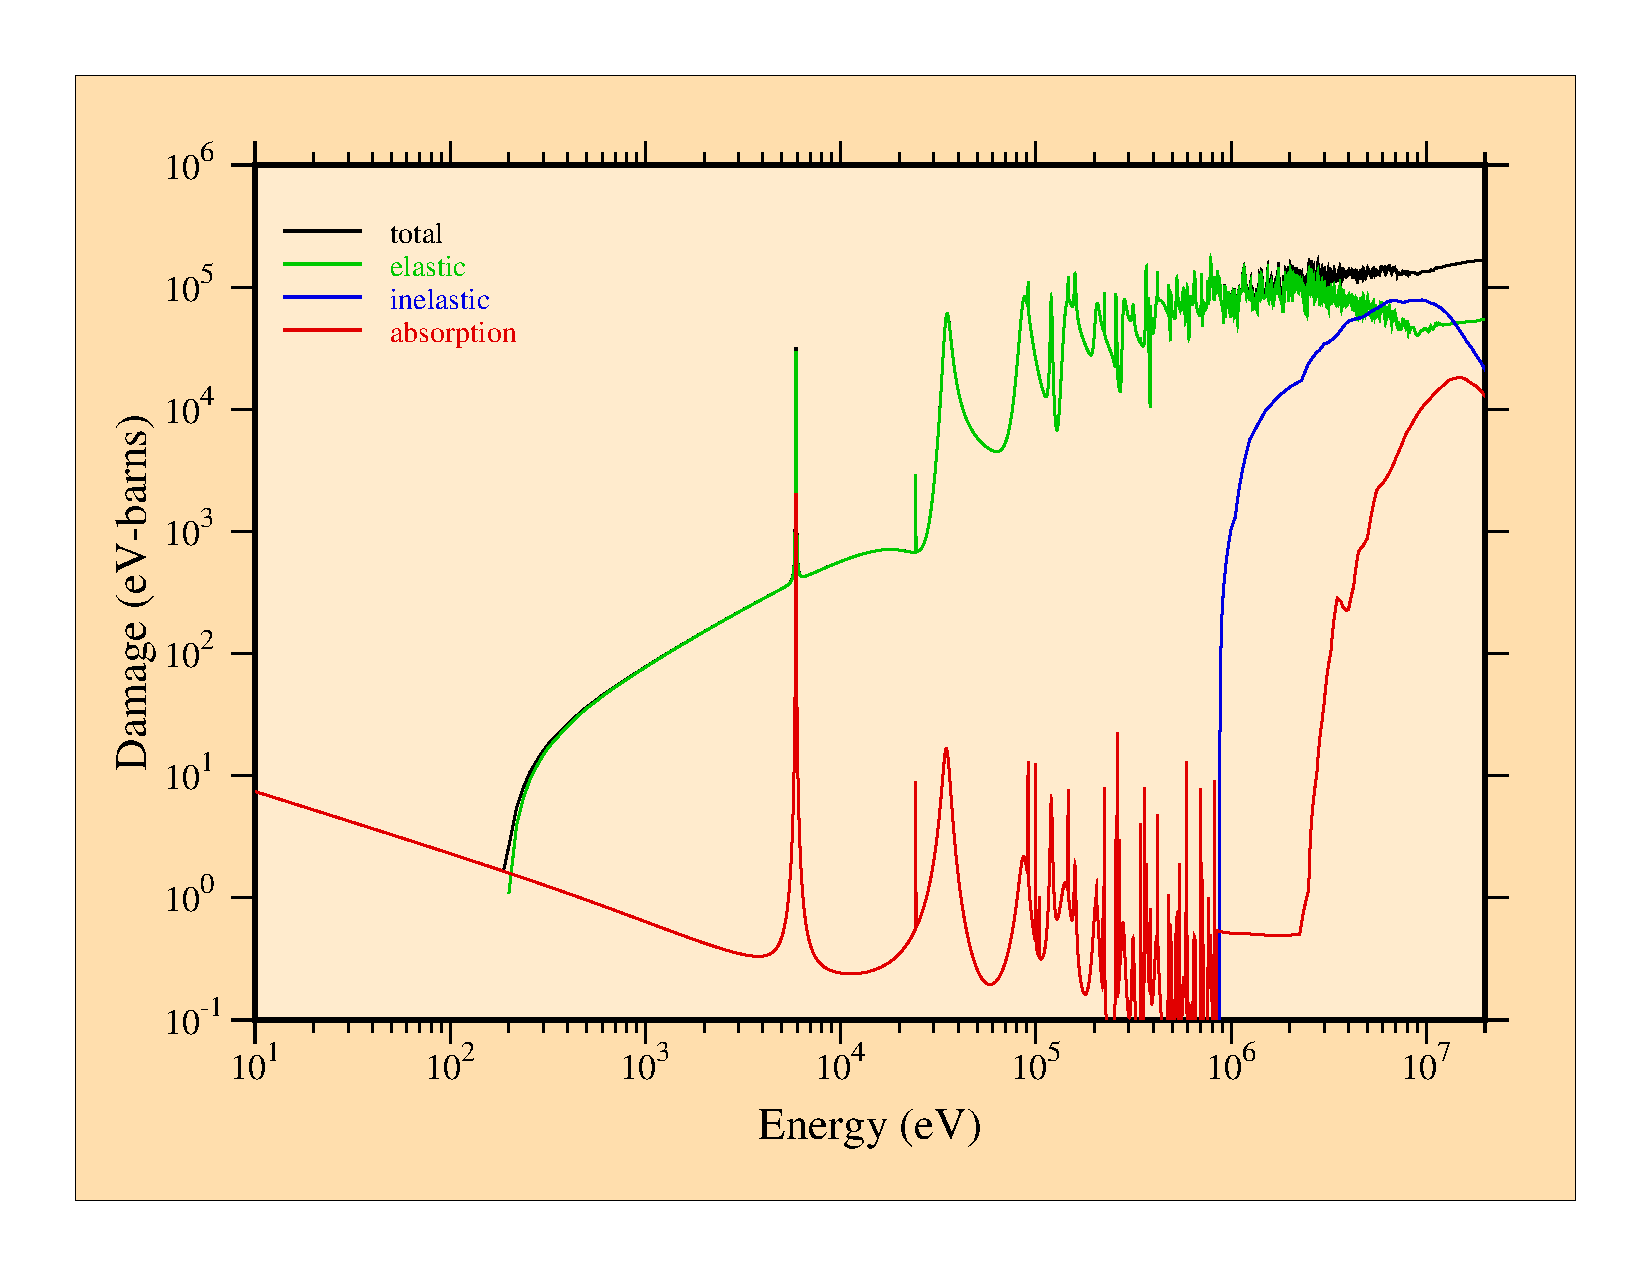
\includegraphics[keepaspectratio,height=3.2in, angle=0]{figs/heatr3ack}
\caption[Components of radiation damage energy production for $^{27}$Al]
{Components of radiation damage energy production
for $^{27}$Al from ENDF/B-VII.0.  Note that capture dominates at
very low energies, then elastic dominates, and finally inelastic
begins to contribute at very high energies.}
\label{f3}
\end{figure}

Fig.~\ref{f3} gives a typical result for a damage energy
production calculation, showing the separate contributions of
elastic, inelastic, and absorption processes.

\subsection{Heating and Damage from File 6}
\label{ssHEATR_file6}

A number of the evaluations in ENDF/B-VI and later include complete
energy-angle distributions for all of the particles produced
by a reaction, including the residual nucleus\index{recoil distributions}.
In these cases, HEATR can compute the contributions to KERMA by
calculating the average energy in the spectrum of each outgoing
charged particle or residual nucleus and using Eq.~\ref{direct}.

A fully-populated section of File 6 contains subsections for all of
the particles and photons produced by the reaction, including
the recoil nucleus.  There are a number of different schemes
used to represent the energy-angle distributions for these
outgoing particles.  The most important ones for HEATR follow:
\begin{itemize}
\begin{singlespace}
\item {\it No distribution}.  In this case, the subsection is
      inadequate for use in heating and damage calculations.
      A warning message is issued.

\item {\it Two-body angular distribution}.  These are basically
      the same as distributions in File 4.

\item {\it Recoil distribution}.  This particle is a recoil
      nucleus from a two-body reaction.  Its angular
      distribution is assumed to be the complement of the
      angular distribution for the \underbar{first} subsection
      in this section.

\item {\it CM Kalbach distribution}.  This format is often used
      by LANL evaluations, and transformation to the
      laboratory frame is required.  The looping order for
      the data is $E$, $E'$, $\mu$.

\item{\it LAB Legendre distribution}.  This format is used in
      most of the ORNL evaluations for ENDF/B-VI.  It is
      already in the laboratory frame, and the angular
      information can be simply ignored.

\item{\it LAB angle-energy distribution}.  This format is
      used for the $^{9}$Be evaluation of ENDF/B-VI by LLNL.
      The looping order is $E$, $\mu$, $E'$.
\end{singlespace}
\end{itemize}

\noindent
The normal procedure is to loop through all of these subsections.
The subsections producing neutrons are processed to be used in
a total energy check, but they contribute nothing to the heating
or to the damage. Subsections describing charged particles and
residual nuclei are processed into heating and damage contributions.
Finally, the photon subsection is processed for the photon energy
check and the total energy check, even though it does not affect
either heating or damage.  Any remaining difference between the
eV-barns available for the reaction and the eV-barns carried
away by the neutrons, photons, particles, and recoil is added
into the heating to help preserve the total energy deposition
in the spirit of the energy-balance method.

For ``two-body'' sections,  the emitted particle energy is given by

\begin{equation}
   E'=\frac{A'E}{A+1}\Bigl(1+2R\mu+R^2\Bigr) \,\,,
\label{ebar6}
\end{equation}
\vspace{1 pt}

\noindent
where

\begin{equation}
   R=\sqrt{\frac{A(A+1-A')}{A'}} \,\,,
\label{beta}
\end{equation}

\noindent
and $A'$ is the ratio of the mass of the outgoing particle to
that of the incident particle.  The heating is obtained by doing
a simple integral over $\mu$, and the damage is computed using
the integral over $\mu$ given in Eq.~\ref{damint}.  In both
cases, the integrals are performed using either a 20-point
Gauss-Legendre quadrature\index{Gauss-Legendre quadrature}
(for Legendre representations) or a trapezoidal integration
(for tabulated data).

For ``recoil'' sections, the code backs up to the particle
distribution and calculates the recoil using  the same method
described above with the sign of $\mu$ changed.

For laboratory distributions that use the $E$, $E'$, $\mu$
ordering, the angular part can be ignored, and the heating and
damage become

\begin{equation}
   K(E)=\int g(E{\rightarrow}E')E'\,dE'\,\,,
\label{KofE}
\end{equation}

\noindent
and

\begin{equation}
   D(E)=\int g(E{\rightarrow}E')P(E')\,dE'\,\,,
\label{DofE}
\end{equation}

\noindent
where $g(E{\rightarrow}E')$ is the angle-integrated energy
distribution from File 6, and $P(E')$ is the damage partition
function.  Trapezoidal integration is used for the continuum,
and the integrand is simply added into the sum for the
delta functions (if any).

Heating for subsections that use the ordering $E$, $\mu$, $E'$
is computed using the formula

\begin{equation}
   K(E)=\int \left\{ \int g(E{\rightarrow}E',\mu)
     E'\,dE'\right\} d\mu\,\,,
\label{llnl}
\end{equation}

\noindent
where an inner integral is performed using trapezoidal
integration for each value in the $\mu$ grid.  The results
are then used in a second trapezoidal integration over $\mu$.
The damage integral is performed at the same time in a
parallel manner.

The problem is somewhat more difficult for subsections
represented in the center-of-mass frame.  The definitions
for $K(E)$ and $D(E)$ are the same as those given above,
except that the quantity $g(E{\rightarrow}E')$ has to be
generated in the lab system.  The methods used to do the
transformation are basically the same in HEATR and
\hyperlink{sGROUPRhy}{GROUPR}\index{GROUPR}.  The
first step is to set up an adaptive
integration over $E'$.  The first value needed to prime the
stack is obtained by calling \cword{h6cm} with $E'{=}0$.  It
returns the corresponding value of $g$ in the lab system and
a value for \cword{epnext}.  The second value for the stack is
computed for $E$=\cword{epnext}.  The routine then subdivides
this interval until 2\% convergence is achieved, accumulating
the contributions to the heating and damage integrals as it
goes.  It then moves up to a new panel.  This process
continues until the entire range of $E'$ has been covered.

The key to this process is \cword{h6cm}\index{h6cm@{\ty h6cm}}.
As described in more detail in the
\hyperlink{sGROUPRhy}{GROUPR}\index{GROUPR} chapter
of this manual, it performs integrals of the form

\begin{equation}
   g_L(E{\rightarrow}E'_L)=\int_{\mu_{\rm min}}^{+1}
      g_C(E{\rightarrow}E'_C,\mu_C)\,J\,d\mu_L\,\,,
\label{transCM}
\end{equation}

\noindent
where $L$ and $C$ denote the laboratory and center-of-mass
systems, respectively, and $J$ is the Jacobian for the
transformation.  The contours in the $E'_C$,$\mu_C$ frame that
are used for these integrals have constant $E'_L$.  The
limiting cosine, $\mu_{\rm min}$, depends on kinematic factors
and the maximum possible value for $E'_C$ in the File 6
tabulation.

The ENDF/B-VII\index{ENDF!ENDF/B-VII} library contains a few
abbreviated versions of File 6\index{File 6} that contain an
energy-angle distribution for neutron emission, but no
recoil or photon data.  In order to get semi-reasonable
results for both heating and damage for such cases, HEATR
applies a ``one-particle recoil approximation,''
where the first particle emitted is assumed to induce all
the recoil.  There are also some cases where capture photons
are described in MF=6/MT=102 with no corresponding recoil data.
Here, the recoil can be added using the same logic described
above for capture represented using File 15.  The difference
between the eV-barns available for the reaction and the energy
accounted for by the emitted neutrons, photons, particles, and
the approximated recoil is added into the heating in order to
preserve the total heating in the spirit of the energy-balance
method.


\subsection{User Input}
\label{ssHEATR_inp}

The input instructions that follow were reproduced from the
comment cards in the current version of HEATR.
\index{HEATR!HEATR input}
\index{input!HEATR}

\small
\begin{ccode}

   !---input specifications (free format)------------------------
   !
   ! card 1
   !    nendf    unit for endf tape
   !    nin      unit for input pendf tape
   !    nout     unit for output pendf tape
   !    nplot    unit for graphical check output
   ! card 2
   !    matd     material to be processed
   !    npk      number of partial kermas desired (default=0)
   !    nqa      number of user q values (default=0)
   !    ntemp    number of temperatures to process
   !             (default=0, meaning all on pendf)
   !    local    0/1=gamma rays transported/deposited locally
   !             (default=0)
   !    iprint   print (0 min, 1 max, 2 check) (default=0)
   !    ed       displacement energy for damage
   !             (default from built-in table)
   ! card 3      for npk gt 0 only
   !    mtk      mt numbers for partial kermas desired
   !             total (mt301) will be provided automatically.
   !             partial kerma for reaction mt is mt+300
   !             and may not be properly defined unless
   !             a gamma file for mt is on endf tape.
   !             special values allowed--
   !               303   non-elastic (all but mt2)
   !               304   inelastic (mt51 thru 91)
   !               318   fission (mt18 or mt19, 20, 21, 38)
   !               401   disappearance (mt102 thru 120)
   !               442   total ev-barns
   !               443   total kinematic kerma (high limit)
   !             damage energy production values--
   !               444   total
   !               445   elastic (mt2)
   !               446   inelastic (mt51 thru 91)
   !               447   disappearance (mt102 thru 120)
   !          cards 4 and 5 for nqa gt 0 only
   ! card 4
   !    mta      mt numbers for users q values
   ! card 5
   !    qa       user specified q values (ev)
   !               (if qa.ge.99.e6, read in variable qbar
   !                  for this reaction)
   ! card 5a     variable qbar (for reactions with qa flag only)
   !    qbar      tab1 record giving qbar versus e (1000 words max)
   !
   !----------------------------------------------------------------

\end{ccode}
\normalsize

Card 1 specifies the input and output units for HEATR.  They
are all ENDF-type files.  The input PENDF file has normally
been through \hyperlink{sRECONRhy}{RECONR} and
\hyperlink{sBROADRhy}{BROADR}, but it is possible to run HEATR
directly on an ENDF file in order to do kinematic checks.  In
this case, the results in the resonance range should be
ignored. Defining \cword{nplot} will produce a file of input
for the \hyperlink{sVIEWRhy}{VIEWR}\index{VIEWR} module
containing detailed energy-balance
test results.  This option should only be used together with
\cword{iprint}=2.

On Card 2, the default value for \cword{npk} is zero, which
instructs the code to process the energy-balance total KERMA
(MT=301) only.  Most often, the user will also want to include MT=443
and MT=444 (\cword{npk}=2).  The kinematic KERMA computed
when MT=443 is requested is very useful for judging the
energy-balance consistency\index{energy balance consistency}
of an evaluation (see the subsection on ``Diagnosing
Energy-Balance Problems'', Section~\ref{ssHEATR_EB_Prob},
below).  It can also be used instead
of the energy-balance value in MT=301 when local heating effects
are important and the evaluation scores poorly in an energy-balance
check.  Damage energy production cross sections (MT=444) should be
computed for important structural materials; this expensive
calculation can be omitted for other materials.

When kinematic checks are desired, a number of additional
\cword{npk} values can be included.  They can be determined by
checking the evaluation to see what partial KERMA factors are
well defined.  For old-style evaluations that do not use File 6,
look for the MT values used in Files 12 and 13.  Many
evaluations use only MT=3 and MT=102 (or 3, 18, and 102 for
fissionable materials); in these cases, the only \cword{mtk}
values that make sense are 302, 303, and 402 (or 302, 303, 318,
and 402 for fissionable materials).  Caution: in many evaluations,
MT=102 is used at low energies and taken to zero at some
breakpoint.  MT=3 is used at higher energies.  In these
evaluations, the partial KERMA MT=402 does not make sense above
the breakpoint, and MT=3 does not make sense below it.

More complicated photon-production evaluations may include MT=4
and/or discrete-photon data in MT=51-90.  In these cases, the
user can request \cword{mtk}=304.  The same kind of energy-range
restriction discussed for MT=102 can occur for the inelastic
contributions.  Other evaluations give additional partial
reactions that can be used to check the photon production and
energy-balance consistency of an evaluation in detail.  HEATR
can handle 6 additional reactions at a time.  Multiple runs
may be necessary in complex cases.

Note that several special \cword{mtk} values are provided for
the components of the damage-energy production cross section.
They were used to prepare Fig.~\ref{f3}, and may be of interest
to specialists, but they are not needed for most libraries.

In a few cases in the past, it has been necessary to change
the $Q$-values that are normally retrieved from the ENDF tape.
In addition, it is sometimes necessary to replace the single
$Q$-value supplied in MF=3 with an energy-dependent Q function
for an element.  One example of the former occurred for $^{16}$O
for ENDF/B-V.  The first inelastic level (MT=51) decays by
pair production rather than the more normal mode of photon
emission.  In order to get the correct heating, it was necessary
to change the $Q$-value by giving Card 4 and Card 5 as follows:

\small
\begin{ccode}

   51
   -5.0294e6

\end{ccode}
\normalsize

\noindent
That is, the $Q$-value is increased by twice the electron energy
of 0.511 MeV.  Another example is the sequential (n,2n)
reaction for $^{9}$Be in ENDF/B-V.  It is necessary to include
4 changes to the $Q$-values:

\small
\begin{ccode}

   46 47 48 49/
   -1.6651e6 -1.6651e6 -1.6651e6 -1.6651e6/

\end{ccode}
\normalsize

\noindent
The next example illustrates using energy-dependent $Q$-values
\index{energy-dependent Q} for elemental titanium.  Set
\cword{nqa} equal to 3 and give the following values on
Cards 4, 5, and 5a:

\small
\begin{ccode}

   16 103 107/
   99e6 99e6 99e6/
   0. 0. 0 0 1 8
   8 2
   8.0e6 -8.14e6 9.0e6 -8.14e6 1.1e7 -8.38e6
   1.2e7 -8.74e6 1.3e7 -1.03e7 1.4e7 -1.091e7
   1.5e7 -1.11e7 2.0e7 -1.125e7/
   0. 0. 0 0 1 9
   9 2
   1.0e-5 1.82e5 4.0e6 1.82e5 5.0e6 -1.19e6
   6.0e6 -2.01e6 7.0e6 -2.20e6 8.0e6 -2.27e6
   1.4e7 -2.35e6 1.7e6 -2.43e6 2.0e7 -2.37e6/
   0. 0. 0 0 1 9
   9 2
   1.0e-5 2.182e6 6.0e6 2.182e6 7.0e6 2.10e6
   8.0e6 -3.11e5 9.0e6 -9.90e5 1.0e7 -1.20e6
   1.1e7 -1.27e6 1.4e6 -1.32e6 2.0e7 -1.48e6/

\end{ccode}
\normalsize

The next parameter on Card 2 is \cword{ntemp}.  For normal
runs, use zero, and all the temperatures on the input PENDF
tape will be processed.  For kinematic check runs, use
\cword{ntemp}=1.  The \cword{local} parameter suppresses
the processing of the photon-production files, if any.
The photon energy appears in the KERMA factors as if the
photons had very short range.  A useful way to use the
\cword{iprint} parameter is to set it to zero for normal
runs, which produce heating and damage values at all
temperatures, and to use \cword{iprint}=2 for the
energy-balance check run, which is performed for the first
temperature on \cword{nin} only.

Card 3 gives the partial KERMA and damage selection MT
numbers.  Note that the user does not include MT=301 in this
list.  It is always inserted as the first value automatically.
Giving MT=301 in this list will cause an informative message
to be issued.

Cards 4, 5, and 5a give the user's changes to the ENDF Q
values.  The way in which to use these cards was described
in connection with \cword{nqa} on Card 2.

\subsection{Reading HEATR Output}
\label{ssHEATR_output}

When full output and/or kinematic checks have been requested,
\index{HEATR!HEATR output}
HEATR loops through the reactions found in Files 3, 12, and 13.
For each reaction, it prints out information about the energies,
yields, cross sections, and contributions to heating.
The energy grid used is a subset of the PENDF grid.
At present, decade steps are used below 1 eV, factor-of-two
steps are used from 1 eV to 100 keV, quarter-lethargy steps
are used above 100 keV, and approximately 1 MeV steps are used
above 2 MeV.  An example of this printout for elastic scattering
in ENDF/B-VII.0 $^{27}$Al is shown below:

\small
\begin{ccode}

 neutron heating for mt  2   q0 =  0.0000E+00     q =  0.0000E+00
            e          ebar   ...       xsec       heating        damage
   1.0000E-05    9.3052E-06   ... 1.5694E+01    1.0903E-05    0.0000E+00
   1.0000E-04    9.3052E-05   ... 5.1179E+00    3.5557E-05    0.0000E+00
   1.0000E-03    9.3052E-04   ... 2.0644E+00    1.4342E-04    0.0000E+00
   1.0000E-02    9.3052E-03   ... 1.4925E+00    1.0369E-03    0.0000E+00
   1.0000E-01    9.3052E-02   ... 1.4318E+00    9.9474E-03    0.0000E+00
     ...
   1.0000E+03    9.3052E+02   ... 1.3662E+00    9.4914E+01    7.7171E+01
   2.0000E+03    1.8610E+03   ... 1.3196E+00    1.8337E+02    1.5115E+02
   5.0000E+03    4.6526E+03   ... 1.2130E+00    4.2136E+02    3.3998E+02
   1.0000E+04    9.3052E+03   ... 1.0367E+00    7.2028E+02    5.6725E+02
   2.0000E+04    1.8610E+04   ... 6.6204E-01    9.1991E+02    7.0347E+02
   5.0000E+04    4.6526E+04   ... 2.3220E+00    8.0660E+03    5.8732E+03
   1.0000E+05    9.3052E+04   ... 5.2976E+00    3.6805E+04    2.5521E+04
     ...
   1.0000E+07    9.7233E+06   ... 7.4942E-01    2.0738E+05    4.5689E+04
   1.1000E+07    1.0699E+07   ... 7.4953E-01    2.2576E+05    4.7347E+04
   1.2000E+07    1.1682E+07   ... 7.6363E-01    2.4286E+05    4.9202E+04
   1.3000E+07    1.2673E+07   ... 7.6329E-01    2.4980E+05    4.9559E+04
   1.4000E+07    1.3670E+07   ... 7.7918E-01    2.5737E+05    5.0566E+04
   1.5000E+07    1.4671E+07   ... 7.9297E-01    2.6088E+05    5.1189E+04
   1.6000E+07    1.5676E+07   ... 8.1414E-01    2.6347E+05    5.1973E+04
   1.7000E+07    1.6681E+07   ... 8.3429E-01    2.6577E+05    5.2680E+04
   1.8000E+07    1.7689E+07   ... 8.4524E-01    2.6246E+05    5.2747E+04
   1.9000E+07    1.8695E+07   ... 8.7093E-01    2.6568E+05    5.3787E+04
   2.0000E+07    1.9703E+07   ... 8.9326E-01    2.6547E+05    5.4573E+04
     ...
   1.4000E+08    1.3985E+08   ... 2.9730E-01    4.3523E+04    1.4994E+04
   1.4600E+08    1.4585E+08   ... 2.7580E-01    4.1851E+04    1.3890E+04
   1.5000E+08    1.4984E+08   ... 2.6510E-01    4.1161E+04    1.3339E+04

\end{ccode}
\normalsize

\noindent
Note the identification and Q information printed on the first
line; \cword{q} is the ENDF $Q$-value from File 3, and \cword{q0} is
the corresponding mass-difference $Q$-value needed for Eq.~\ref{kij}.
The \cword{ebar}, \cword{yield} (which was replaced by ``...''
to make this listing fit better), and \cword{xsec} columns contain
$\overline{E}_n$, $Y$, and $\sigma$, respectively.   The
\cword{heating} column is just $(E{+}Q{-}Y\overline{E}_n)\sigma$.
The results are similar for discrete inelastic levels represented
using File 4.  The heating due to the associated photons will be
subtracted later while MF=12 or MF=13 is being processed.  However,
if an LR flag is set, the residual nucleus from the (n,n$'$)
reaction breaks up by emitting additional particles.  This extra
breakup energy changes the \cword{q0} value.  An example of such
a section for $^{27}$Al(n,n$_{25}$)p from ENDF/B-V follows:

\small
\begin{ccode}

 neutron heating for mt 75   q0 = -8.2710e+06     q = -1.0750e+07
              e          ebar         yield          xsec       heating
     1.2000e+07    7.8653e+05    1.0000e+00    8.2242e-02    2.4199e+05
     1.3000e+07    1.7116e+06    1.0000e+00    8.0121e-02    2.4176e+05
     1.4000e+07    2.6427e+06    1.0000e+00    5.9282e-02    1.8296e+05
     1.5000e+07    3.5864e+06    1.0000e+00    4.1834e-02    1.3147e+05
     1.6000e+07    4.5096e+06    1.0000e+00    2.8880e-02    9.2977e+04
     1.7000e+07    5.4335e+06    1.0000e+00    1.9867e-02    6.5472e+04
     1.8000e+07    6.3848e+06    1.0000e+00    1.3677e-02    4.5739e+04
     1.9000e+07    7.2944e+06    1.0000e+00    9.4771e-03    3.2550e+04
     2.0000e+07    8.2479e+06    1.0000e+00    6.6142e-03    2.3025e+04

\end{ccode}
\normalsize

\noindent
Starting with ENDF/B-VI, discrete-inelastic sections may also be
given in File 6.  Such sections contain their own photon
production data, and the \cword{heating} column will represent
the entire recoil energy as in Eq.~\ref{disc}.
(See below for detailed discussion of ENDF/B-VI output.)

For continuum reactions that use MF=4 and MF=5, such as (n,n$'$) or
(n,2n), the neutron part of the display looks like this:

\small
\begin{ccode}

 neutron heating for mt 16   q0 = -1.3057e+07     q = -1.3057e+07
              e          ebar         yield          xsec       heating
     1.4000e+07    1.9960e+05    2.0000e+00    2.4000e-02    1.3051e+04
     1.5000e+07    6.6850e+05    2.0000e+00    1.2320e-01    7.4659e+04
     1.6000e+07    1.0855e+06    2.0000e+00    2.0710e-01    1.5987e+05
     1.7000e+07    1.4308e+06    2.0000e+00    2.6510e-01    2.8667e+05
     1.8000e+07    1.6379e+06    2.0000e+00    3.0300e-01    5.0518e+05
     1.9000e+07    1.7659e+06    2.0000e+00    3.3000e-01    7.9567e+05
     2.0000e+07    1.8755e+06    2.0000e+00    3.5000e-01    1.1172e+06

\end{ccode}
\normalsize

\noindent
Once again, the photon effects will be subtracted later.

Absorption reactions such as (n,$\gamma$) or (n,p), lead to
similar displays, but the particle \cword{ebar} columns will
always be set to zero (no emitted neutrons).  An example
follows:

\small
\begin{ccode}

 neutron heating for mt103   q0 = -1.8278e+06     q = -1.8278e+06
              e          ebar         yield          xsec       heating
     2.5000E+06    0.0000E+00    1.0000E+00    3.2800E-05    2.2048E+01
     3.0000E+06    0.0000E+00    1.0000E+00    1.3300E-03    1.5590E+03
     3.5000E+06    0.0000E+00    1.0000E+00    1.0100E-02    1.6889E+04
     4.0000E+06    0.0000E+00    1.0000E+00    6.9667E-03    1.5133E+04
     4.5000E+06    0.0000E+00    1.0000E+00    1.7000E-02    4.5427E+04
     5.0000E+06    0.0000E+00    1.0000E+00    2.3300E-02    7.3912E+04
        ...
     1.7000E+07    0.0000E+00    1.0000E+00    5.5200E-02    8.3751E+05
     1.8000E+07    0.0000E+00    1.0000E+00    4.7800E-02    7.7303E+05
     1.9000E+07    0.0000E+00    1.0000E+00    4.0200E-02    6.9032E+05
     2.0000E+07    0.0000E+00    1.0000E+00    3.2200E-02    5.8514E+05

\end{ccode}
\normalsize

If File 6 is present (which happens for evaluations in ENDF-6
format only, such as the evaluations in ENDFB-VII), each reaction
will be divided into subsections, one for each emitted particle.
The neutron subsections are displayed as part of the energy-balance
checks, but they do not contribute to KERMA or damage.  The
subsection for each charged particle or residual nucleus will
give the incident energy, average energy for the emitted particle,
cross section, heating contribution, and (optionally) damage
contribution as follows:

\small
\begin{ccode}

 file six heating for mt 28, particle =     1     q =  -8.2721E+06
              e          ebar         yield          xsec       heating
     9.0000E+06    1.2303E+05    1.0000E+00    1.0385E-03    0.0000E+00
     1.0000E+07    4.6746E+05    1.0000E+00    1.3526E-02    0.0000E+00
     ...
     1.8000E+07    3.1862E+06    1.0000E+00    3.7721E-01    0.0000E+00
     1.9000E+07    3.4535E+06    1.0000E+00    3.7577E-01    0.0000E+00
     2.0000E+07    3.7207E+06    1.0000E+00    3.7434E-01    0.0000E+00

 file six heating for mt 28, particle =  1001     q =  -8.2721E+06
              e          ebar         yield          xsec       heating
     9.0000E+06    4.5909E+05    1.0000E+00    1.0385E-03    4.7677E+02
     1.0000E+07    8.9616E+05    1.0000E+00    1.3526E-02    1.2121E+04
     ...
     1.8000E+07    3.5193E+06    1.0000E+00    3.7721E-01    1.3275E+06
     1.9000E+07    3.8257E+06    1.0000E+00    3.7577E-01    1.4376E+06
     2.0000E+07    4.1321E+06    1.0000E+00    3.7434E-01    1.5468E+06

 file six heating for mt 28, particle = 12026     q =  -8.2721E+06
              e          ebar         yield          xsec       heating
     9.0000E+06    3.2104E+05    1.0000E+00    1.0385E-03    3.3340E+02
     1.0000E+07    3.8540E+05    1.0000E+00    1.3526E-02    5.2128E+03
     ...
     1.8000E+07    8.0820E+05    1.0000E+00    3.7721E-01    3.0486E+05
     1.9000E+07    8.6147E+05    1.0000E+00    3.7577E-01    3.2372E+05
     2.0000E+07    9.1475E+05    1.0000E+00    3.7434E-01    3.4243E+05

 file six heating for mt 28, particle =     0     q =  -8.2721E+06
              e          ebar         yield          xsec       heating
     9.0000E+06    1.8347E+05    2.8104E-06    1.0385E-03    0.0000E+00
                                                     ebal   -1.8204E+02
     1.0000E+07    4.4913E+05    3.0441E-05    1.3526E-02    0.0000E+00
                                                     ebal   -2.8626E+02
     ...
     1.8000E+07    1.8309E+06    1.2028E+00    3.7721E-01    0.0000E+00
                                                     ebal    4.5397E+03
     1.9000E+07    1.8856E+06    1.3695E+00    3.7577E-01    0.0000E+00
                                                     ebal    1.8336E+03
     2.0000E+07    1.9403E+06    1.5363E+00    3.7434E-01    0.0000E+00
                                                     ebal   -7.6798E+03

\end{ccode}
\normalsize

\noindent
Note that the last subsection in this example was for emitted
photons.  Photons do not contribute to the KERMA or damage, but
this information is used to check the total energy conservation
for this reaction.  The \cword{ebal} lines show the difference
between the available energy and the sum over all the outgoing
particles. The values should be a small percentage of the total
heating.  If the \cword{ebal} values are too large, there may be
an error in the evaluation, or it may be necessary to refine the
energy grids in the distributions.  In addition, this photon
production information is needed later for the photon energy check.

After all the sections corresponding to MT numbers in File 3
have been processed (using the File 4, File 4/5, or File 6
method as appropriate), the photon production sections in
Files 12 and 13 are processed, if present.  File 12 data are
usually present for radiative capture (MT=102), at least at low
energies.  Simple files normally give a tabulated photon spectrum.
The display gives the average energy for this spectrum in the
\cword{ebar} column and the negative contribution to the
heating computed with Eq.~\ref{cfix} in the \cword{heating}
column.  The \cword{edam} column contains the
$\overline{E^2_\gamma}$ term needed to compute the photon
contribution to the damage, which is given in the \cword{damage}
column.  See Eq.~\ref{D102}.  The display also has an extra
line for each incident energy containing the percent error
``\cword{--- pc}'' between the total photon energy as computed
from File 12 and the value $E{+}Q{-}E/(A{+1})$ computed
from File 3.  As discussed above, HEATR does not guarantee energy
balance in large systems if this error occurs.  The following
example shows some large errors due to mistakes in the ENDF/B-V
evaluation for $^{55}$Mn.  Two columns labeled \cword{edam} and
\cword{xsec} have been removed to show the \cword{heating} and
\cword{damage} columns.  The text has also been shifted to the
left of its normal position to fit better on the printed page.

\small
\begin{ccode}

 photon energy (from yields) mf12, mt102
          e    ebar/err        egam ...      yield     heating      damage
 1  continuum gammas
 1.0000e-05  4.5088e+06  2.4237e+02 ... 2.4791e+00 -4.8477e+09  5.4975e+04
 1.0000e-05    53.7 pc
 1.0703e-04  4.5088e+06  2.4237e+02 ... 2.4791e+00 -1.4819e+09  1.6806e+04
 1.0703e-04    53.7 pc
 1.2520e-03  4.5088e+06  2.4237e+02 ... 2.4791e+00 -4.3347e+08  4.9159e+03
 1.2520e-03    53.7 pc
   ...
 1.3571e+04  4.4522e+06  2.3887e+02 ... 2.4836e+00 -7.3869e+03 -1.2406e-01
 1.3571e+04    51.8 pc
 2.7142e+04  4.3957e+06  2.3536e+02 ... 2.4881e+00 -3.7037e+05 -1.6487e+01
 2.7142e+04    49.9 pc
 5.4287e+04  4.2826e+06  2.2834e+02 ... 2.4972e+00 -2.5604e+04 -2.5340e+00
 5.4287e+04    46.0 pc
 1.0858e+05  4.0563e+06  2.1430e+02 ... 2.5154e+00 -1.3327e+04 -2.7289e+00
 1.0858e+05    38.3 pc

\end{ccode}
\normalsize

Many MF=12, MT=102 sections give multiplicities for the production
of discrete photons.  In these cases, HEATR prints out data for
all of the parts, and it provides a sum at the end.  The
balance error is printed with the sum.  The following example shows
a case with discrete photons.  The last two columns have been
removed (\cword{heating}, \cword{damage}), and the text has been
compacted and shifted to the left to fit on the printed page.

\small
\begin{ccode}

  photon energy (from yields) mf12, mt102
           e    ebar/err        egam        edam        xsec       yield
  1   7.7260E+06 ev gamma
  1.0000e-05  7.7260e+06  1.1448e+03  8.9780e+02  1.1677e+01  3.0000e-01
  1.1406e-04  7.7260e+06  1.1448e+03  8.9780e+02  3.4574e+00  3.0000e-01
  1.1406e-03  7.7260e+06  1.1448e+03  8.9780e+02  1.0934e+00  3.0000e-01
    ...
  2.0000e+07  2.7005e+07  1.1448e+03  8.9780e+02  1.0000e-03  3.0000e-01
  2   7.6950e+06 ev gamma
  1.0000e-05  7.6950e+06  1.1356e+03  8.9091e+02  1.1677e+01  5.0000e-02
  1.1406e-04  7.6950e+06  1.1356e+03  8.9091e+02  3.4574e+00  5.0000e-02
    ...
  2.0000e+07  2.6974e+07  1.1356e+03  8.9091e+02  1.0000e-03  5.0000e-02
  3   6.8630e+06 ev gamma
  1.0000e-05  6.8630e+06  9.0330e+02  7.1515e+02  1.1677e+01  1.2000e-03
  1.1406e-04  6.8630e+06  9.0330e+02  7.1515e+02  3.4574e+00  1.2000e-03
  1.1406e-03  6.8630e+06  9.0330e+02  7.1515e+02  1.0934e+00  1.2000e-03
    ...
 89   3.1000e+04 eV gamma
  1.0000e-05  3.1000e+04  1.8430e-02  0.0000e+00  1.1677e+01  2.8884e-01
  1.0000e-05     0.0 pc
  1.1406e-04  3.1000e+04  1.8430e-02  0.0000e+00  3.4574e+00  2.8884e-01
  1.1406e-04     0.0 pc
  1.1406e-03  3.1000e+04  1.8430e-02  0.0000e+00  1.0934e+00  2.8884e-01
  1.1406e-03     0.0 pc
  1.1912e-02  3.1000e+04  1.8430e-02  0.0000e+00  3.3832e-01  2.8884e-01
  1.1912e-02     0.0 pc
    ...
  2.0000e+07  3.1000e+04  1.8430e-02  0.0000e+00  1.0000e-03  2.8884e-01
  2.0000e+07     0.0 pc

\end{ccode}
\normalsize

\noindent
In this case ($^{27}$Al), the capture energy production checks out
perfectly for the sum of all 89 discrete photons.

Other sections using either File 12 or File 13 generate displays
similar to the following:

\small
\begin{ccode}

 photon energy (from xsecs) mf13, mt  3
              e          ebar          xsec        energy       heating
     1  continuum gammas
     2.0000e+05    3.6753e+06    4.2076e-03    1.5464e+04   -1.5464e+04
     4.0500e+05    3.3863e+06    5.2873e-03    1.7904e+04   -1.7904e+04
     6.0031e+05    3.1097e+06    6.4478e-03    2.0051e+04   -2.0051e+04
     8.0182e+05    2.0089e+06    9.3236e-02    1.8730e+05   -1.8730e+05
     1.0000e+06    9.2622e+05    1.7859e-01    1.6541e+05   -1.6541e+05
     1.2000e+06    9.6151e+05    2.8329e-01    2.7239e+05   -2.7239e+05
   ...

\end{ccode}
\normalsize

\noindent
Note that the photon $\overline{E}\sigma$ is simply subtracted from
the \cword{heating} column for each incident energy.

If the partial KERMA \cword{mtk}=443 was requested in the user's
input, HEATR will print out a special section that tests the
total photon energy production against the kinematic limits
(see Section~\ref{ssHEATR_kinematiclimits} above for the formulas used).
An example follows:

\small
\begin{ccode}

 photon energy production check
              e      ev-barns           min           max
     1.0000e-05    9.0215e+07    9.0187e+07    9.0200e+07
     1.1406e-04    2.6712e+07    2.6704e+07    2.6708e+07
     1.1406e-03    8.4479e+06    8.4453e+06    8.4466e+06
     1.1912e-02    2.6138e+06    2.6130e+06    2.6134e+06
     1.2812e-01    7.9895e+05    7.9871e+05    7.9883e+05
     1.2812e+00    2.5211e+05    2.5203e+05    2.5207e+05
     2.6875e+00    1.7420e+05    1.7415e+05    1.7417e+05
     5.5000e+00    1.2186e+05    1.2182e+05    1.2184e+05
     1.1406e+01    8.4662e+04    8.4636e+04    8.4648e+04
     2.4062e+01    5.8231e+04    5.8213e+04    5.8222e+04
     4.9375e+01    4.0614e+04    4.0601e+04    4.0607e+04
     1.0000e+02    2.8522e+04    2.8514e+04    2.8518e+04
   ...
     8.0000e+06    3.8972e+06    3.7964e+06    4.4880e+06
     9.0000e+06    4.4782e+06    4.4401e+06    5.4986e+06
     1.0000e+07    4.9645e+06    5.2078e+06    6.6176e+06
     1.1000e+07    5.3712e+06    6.1302e+06    7.8374e+06   ----
     1.2000e+07    5.3212e+06    5.8699e+06    8.0618e+06
     1.3000e+07    5.0984e+06    5.9333e+06    8.5312e+06   ----
     1.4000e+07    4.7415e+06    5.7172e+06    8.6605e+06   ----
     1.5000e+07    4.0795e+06    4.7419e+06    8.0409e+06   ----
     1.6000e+07    3.2521e+06    3.6806e+06    7.2734e+06   ----
     1.7000e+07    2.8079e+06    2.8418e+06    6.6927e+06
     1.8000e+07    2.7492e+06    2.2915e+06    6.2850e+06
     1.9000e+07    2.9626e+06    1.9674e+06    6.2330e+06
     2.0000e+07    3.4419e+06    1.7938e+06    6.1994e+06

\end{ccode}
\normalsize

\noindent
The low and high kinematic limits\index{kinematic limits}
will be the same at low energies where only kinematics affect
the calculations.  They may be the same for all energies for
ENDF/B-VII evaluations that provide complete distributions
for all outgoing charged particles and recoil nuclei.  Normally,
the limits diverge above the threshold for continuum reactions.
Note that HEATR marks lines where the computed value goes more
than a little way outside the limits with the symbols \cword{++++}
or \cword{----}.  It is often convenient to extract these
numbers from the output listing and plot them (see Fig.~\ref{he4}).
Although the energy grid is a little coarse, such plots can
often be useful (see below).

\begin{figure}[bp]\centering
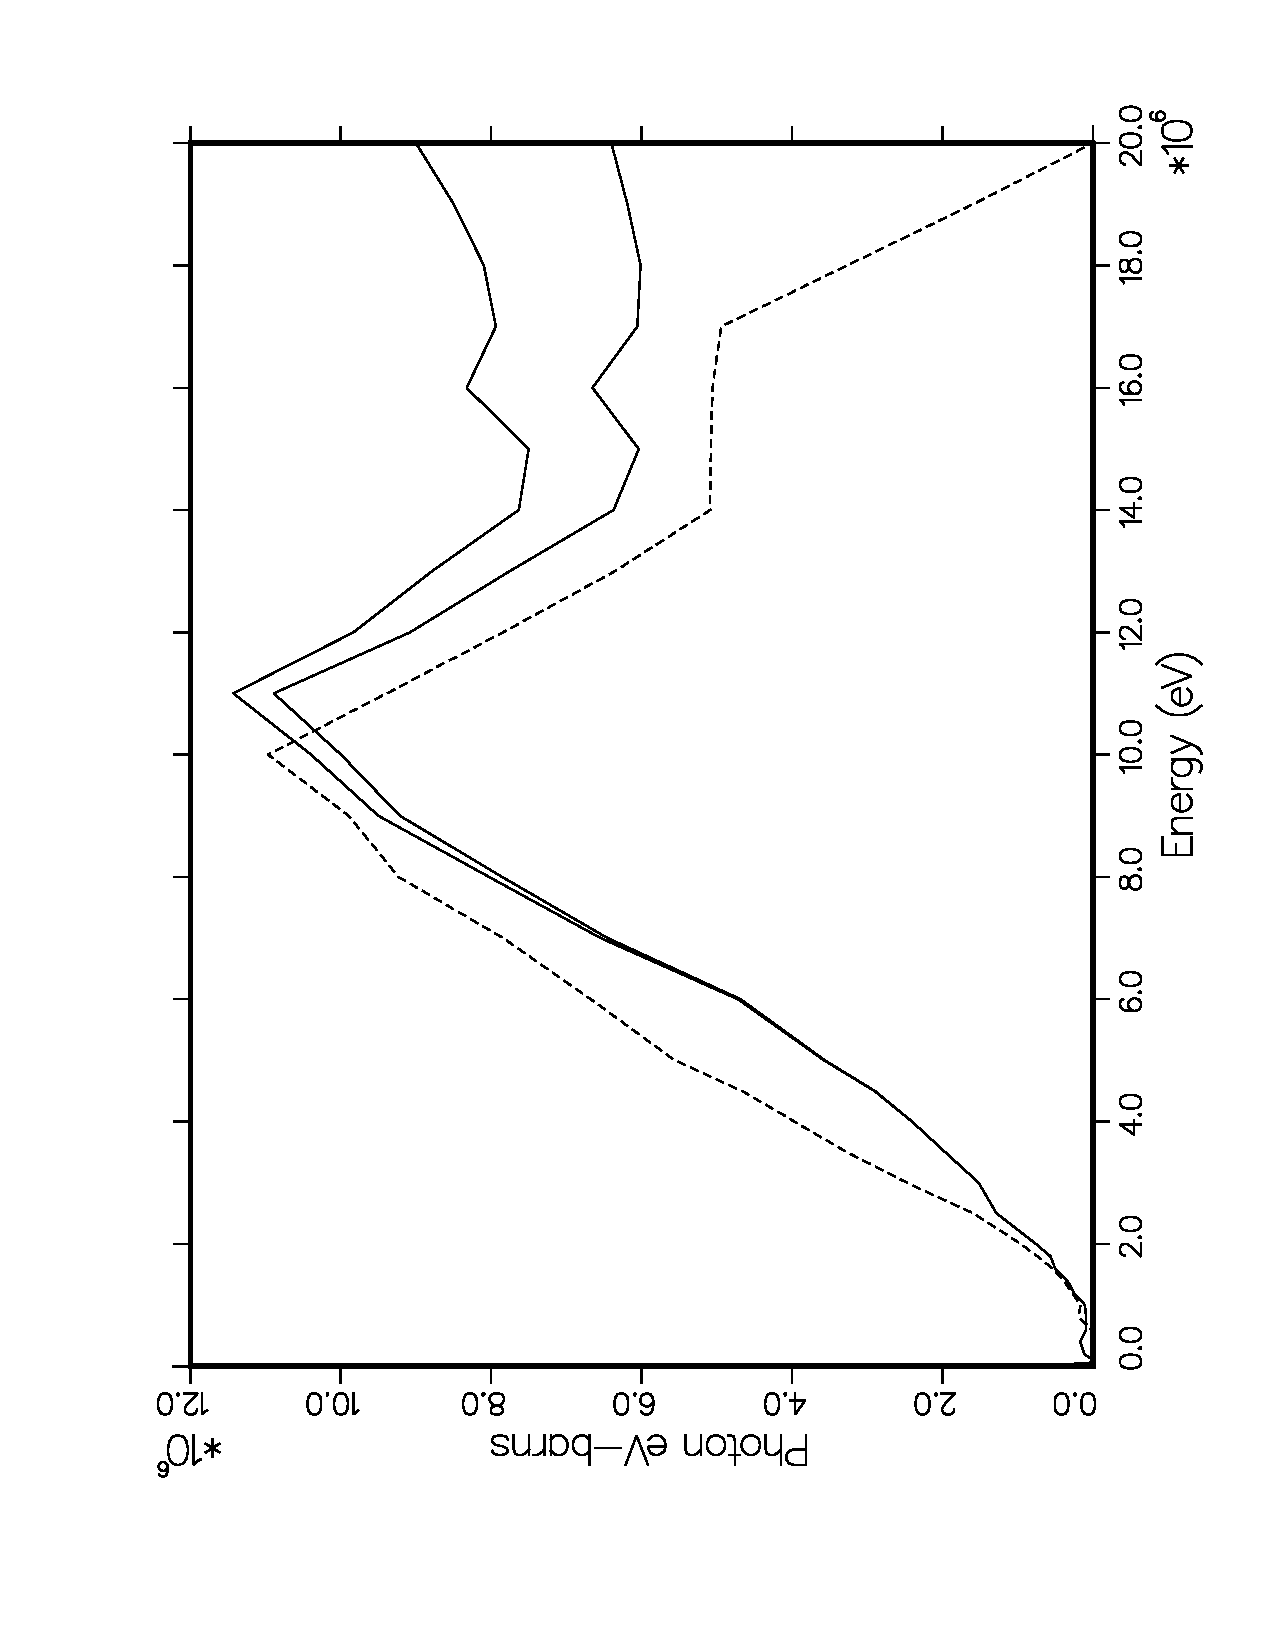
\includegraphics[keepaspectratio,height=3.5in, angle=270]{figs/heatr4ack}
\caption[Total photon energy production and kinematic limits for $^{55}$Mn]
{Example of a plot comparing the total photon energy production for
  $^{55}$Mn from ENDF/B-V.1 (dashed) with the kinematic limits (solid).}
\label{he4}
\end{figure}

The last part of a full HEATR output listing is a tabulation of
the computed KERMA and damage coefficients on the normal coarse
energy grid.  Columns are provided for the total KERMA and
for each of the partial KERMA results requested with \cword{mtk}
values in the user's input.  If kinematic checks were requested,
the check values are written just above and below the corresponding
partial KERMA values.  In addition, \cword{low} and \cword{high}
messages are written just above or just below the kinematic limits
in every column where a significant violation of the limits occurs.
Caution: if summation reactions (MT=3, MT=4) were used to define
the photon production over some parts of the energy range, the
partial KERMA results may not make sense at some energies.  For
example, consider the common pattern in ENDF/B-V where MT=102
is used for capture at low energies, but at higher energies, it
is set to zero, and the capture contribution is included in MT=3
(nonelastic).  Clearly, the partial KERMA MT=402 doesn't make
sense above this breakpoint.  The following example shows part
of the final KERMA listing for ENDF/B-V.1 $^{55}$Mn.  The
damage column was removed and the columns compressed to fit
on the printed page.

\newpage
\small
\begin{ccode}

final kerma factors
          e          301          302          303          402          443

        min   1.2400e-04   3.7775e-06   1.2022e-04   1.2022e-04
 1.0000e-05   4.0068e+05   3.7775e-06   4.0068e+05   4.0068e+05   4.0068e+05
        max   3.3820e+05   3.7775e-06   3.3820e+05   3.3820e+05
                high                      high         high

  ...

        min   3.2373e+04   2.3497e+04   8.8759e+03   4.1114e+01
 6.0031e+05   1.0017e+05   2.3497e+04   7.6673e+04   2.9899e+04   3.2375e+04
        max   3.2375e+04   2.3497e+04   8.8781e+03   4.3366e+01
                high                      high         high

                 low                       low
        min   7.3041e+04   5.9403e+04   1.3638e+04   4.4748e+01
 8.0182e+05  -2.4355e+04   5.9403e+04  -8.3758e+04   2.4987e+04   7.3043e+04
        max   7.3043e+04   5.9403e+04   1.3640e+04   4.6676e+01
                                                        high

                low                       low
        min   9.8973e+04   7.7075e+04   2.1898e+04   4.7777e+01
 1.0000e+06   3.7682e+04   7.7075e+04  -3.9393e+04   2.1917e+04   9.8974e+04
        max   9.8974e+04   7.7075e+04   2.1900e+04   4.9509e+01
                                                        high

                low                       low
        min   1.1397e+05   7.7800e+04   3.6168e+04   4.9760e+01
 1.2000e+06   9.5321e+04   7.7800e+04   1.7521e+04   1.9482e+04   1.1397e+05
        max   1.1397e+05   7.7800e+04   3.6169e+04   5.1335e+01
                                                        high

                low                       low
        min   1.4632e+05   1.0192e+05   4.4402e+04   5.3005e+01
 1.4000e+06   9.8251e+04   1.0192e+05  -3.6667e+03   1.8208e+04   1.4632e+05
        max   1.4632e+05   1.0192e+05   4.4403e+04   5.4511e+01
                                                        high

  ...

        min   2.3650e+05   1.6907e+05   6.7426e+04   1.7607e+02
 1.9000e+07   7.1384e+06   1.6907e+05   6.9693e+06   1.3503e+04   2.5435e+06
        max   2.5435e+06   1.6907e+05   2.3744e+06   1.7939e+02
                high                      high         high

        min   2.4001e+05   1.8261e+05   5.7406e+04   1.4423e+02
 2.0000e+07   9.2369e+06   1.8261e+05   9.0543e+06   1.0908e+04   2.8385e+06
        max   2.8385e+06   1.8261e+05   2.6559e+06   1.4701e+02
                high                      high         high

\end{ccode}
\normalsize

The following subsection discusses how to analyze the ``check''
output of HEATR in order to diagnose energy-balance errors in
ENDF-format evaluations.  The examples are drawn from ENDF/B-V
testing\cite{ebal}.  In general, results like these are less likely to occur
in modern evaluations.

\subsection{Diagnosing Energy-Balance Problems}
\label{ssHEATR_EB_Prob}

The analysis should start with MT=102, because if it is wrong, the
guarantee of energy conservation  for large systems breaks
down.  If the display for MF=12, MT=102 shows messages of the form
``\cword{--- pc}'', there may be a problem.  If these messages only
show up at the higher energies, and if the size of the error
increases with energy, it is probable that the evaluator has
used a thermal spectrum over the entire energy range (this is
very common).  Of course, the total photon energy production
from radiative capture should equal

\begin{equation}
   \frac{A}{A+1}E+Q\,\,,
\end{equation}

\noindent
where the rest of the total energy $E{+}Q$ is carried away by
recoil.  If only a thermal spectrum is given, the $E$ term is
being neglected, and errors will normally appear above about
1 MeV.  The $E$ term can be included in evaluations that use
tabulated data by giving $E$-dependent spectra in File 15; and it
can be included for evaluations that use discrete photons
by setting the ``primary photon'' flags in File 12
properly.  In practice, the capture cross sections above 1 MeV
are often comparatively small due to the $1/v$ tendency of
capture, and the errors introduced by
neglecting the $E$ term can be ignored.

If the MT=102 errors show up at low energies, there is probably
an error in the average photon yield from File 12, in the
average energy computed from File 15, or both.  In the
$^{55}$Mn case shown above, the yield had been incorrectly
entered.  In addition, the spectrum didn't agree with the
experimental data because the bin boundaries were shifted.
Each case must be inspected in detail to find the problems.

The next common source of energy-balance errors in ENDF files
arises from the representation used for inelastic scattering.
Typically, the neutron scattering is described in detail using
up to 40 levels for the (n,n$'$) reaction.  However, the photon
production is often described using MF=13/MT=3 or MF=13/MT=4 and
rather coarse energy resolution.  As a result, it is possible
to find photons for (n,n$_1$) being produced for incident
neutron energies slightly below the MT=51 threshold!  These
photons would lead to a spike of negative KERMA factors.  A
more common effect of the coarse grid used for photon production
is to lead to an underestimate or overestimate of the photon
production by not following the detailed shape of the inelastic
cross section.  The HEATR ``kinematic KERMA'' is correct in
this range since only two-body reactions are active.  Therefore,
a plot of MT=301 and MT=443 on the same frame normally shows
these effects in detail.  Fig.~\ref{he5} is an example of such
a plot.

\begin{figure}[b]\centering
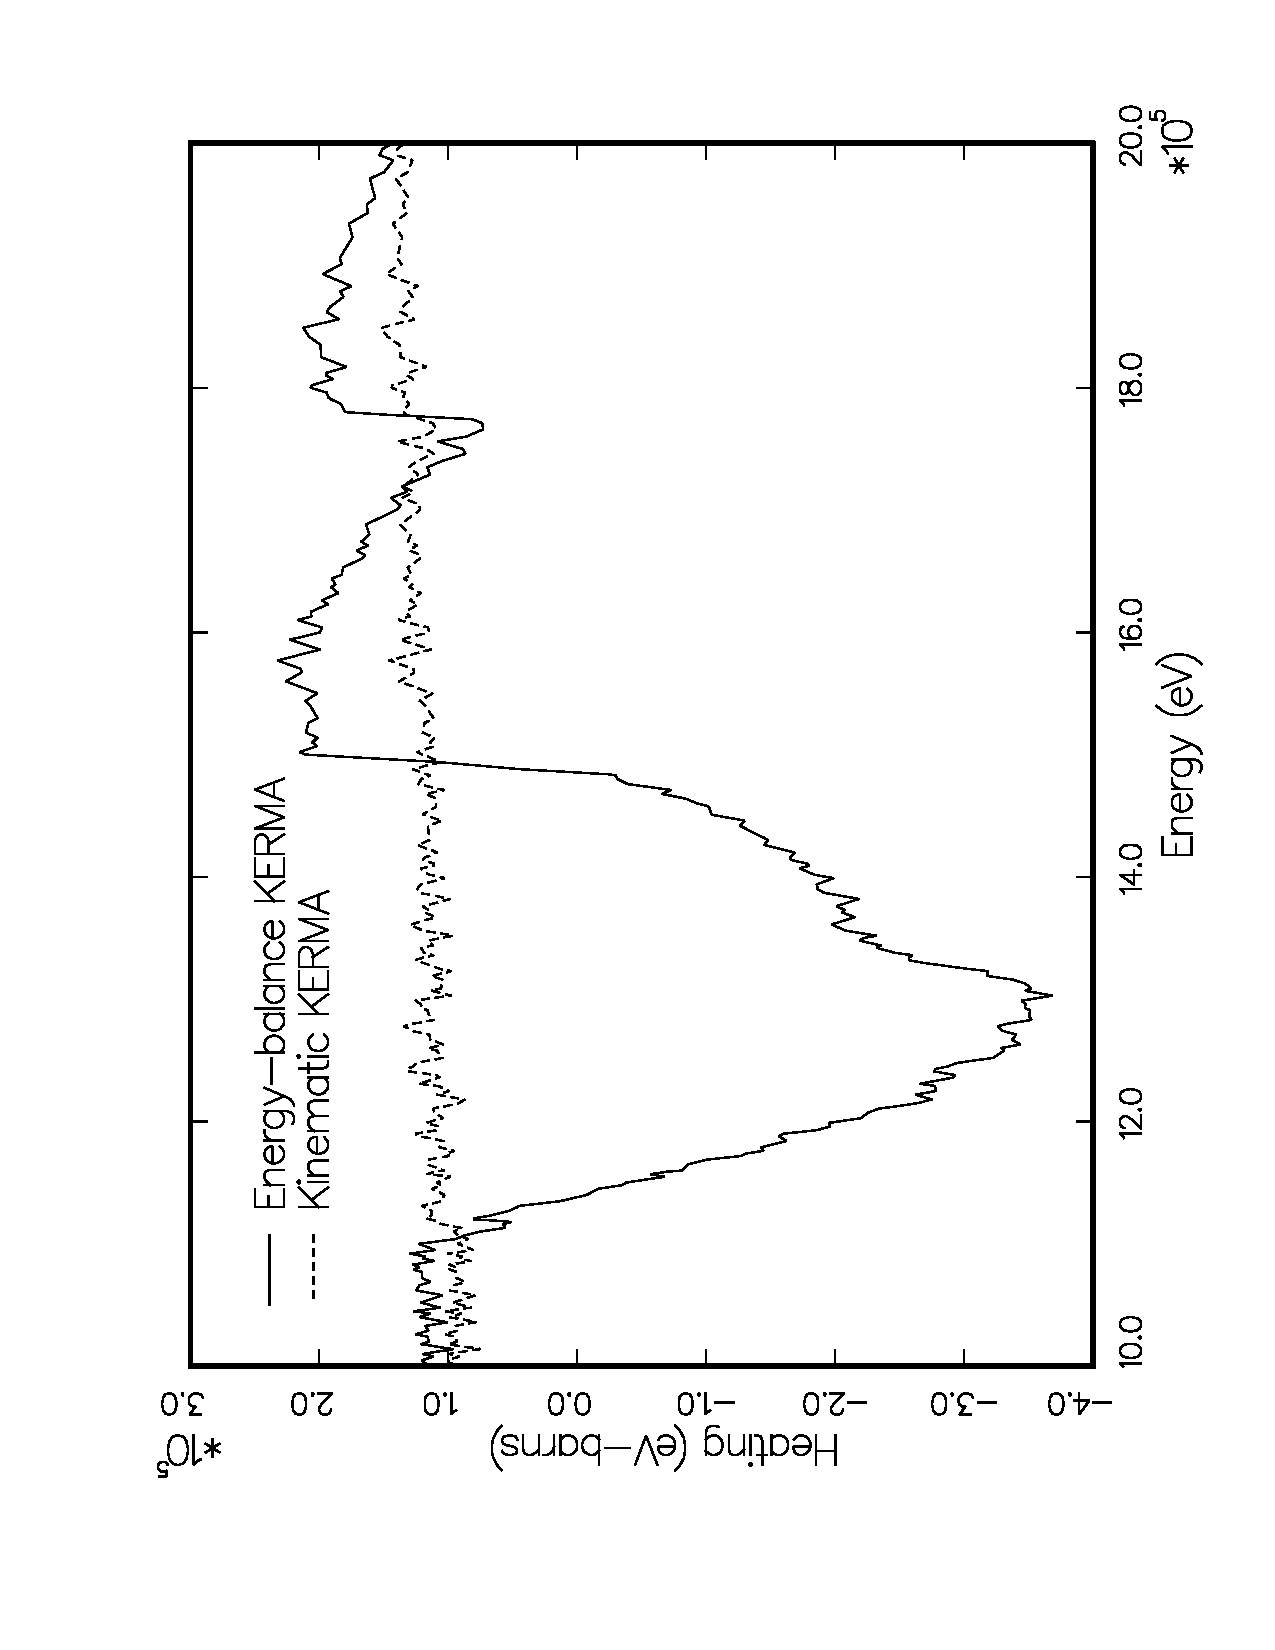
\includegraphics[keepaspectratio,height=3.5in, angle=270]{figs/heatr5ack}
\caption[MT301 and MT443 for $^{59}$Co]{Comparison of MT=301 with
 MT=443 for the region of the discrete-inelastic thresholds for $^{59}$Co
 from ENDF/B-V.2.  Note the large region of negative KERMA.  The best way
 to remove this kind of problem is by using yields in File 12, MT=51, 52, 53,
 \ldots to represent the photon production.}
\label{he5}
\end{figure}

Fig.~\ref{he6} shows both the inelastic cross section
from File 3 and the photon production cross section from File 13
to demonstrate the mismatch in the energy grids that contributes
to the energy-balance errors.  These kinds of errors are best
removed by changing to a representation that uses File 12 to
give photon production yields for the separate reactions MT=51,
MT=52, etc.  This representation makes full use of the File 3
cross sections, and as long as each section of File 12
conserves energy, the total inelastic reaction is guaranteed to
conserve energy, even at the finest energy resolution.

\begin{figure}[t]\centering
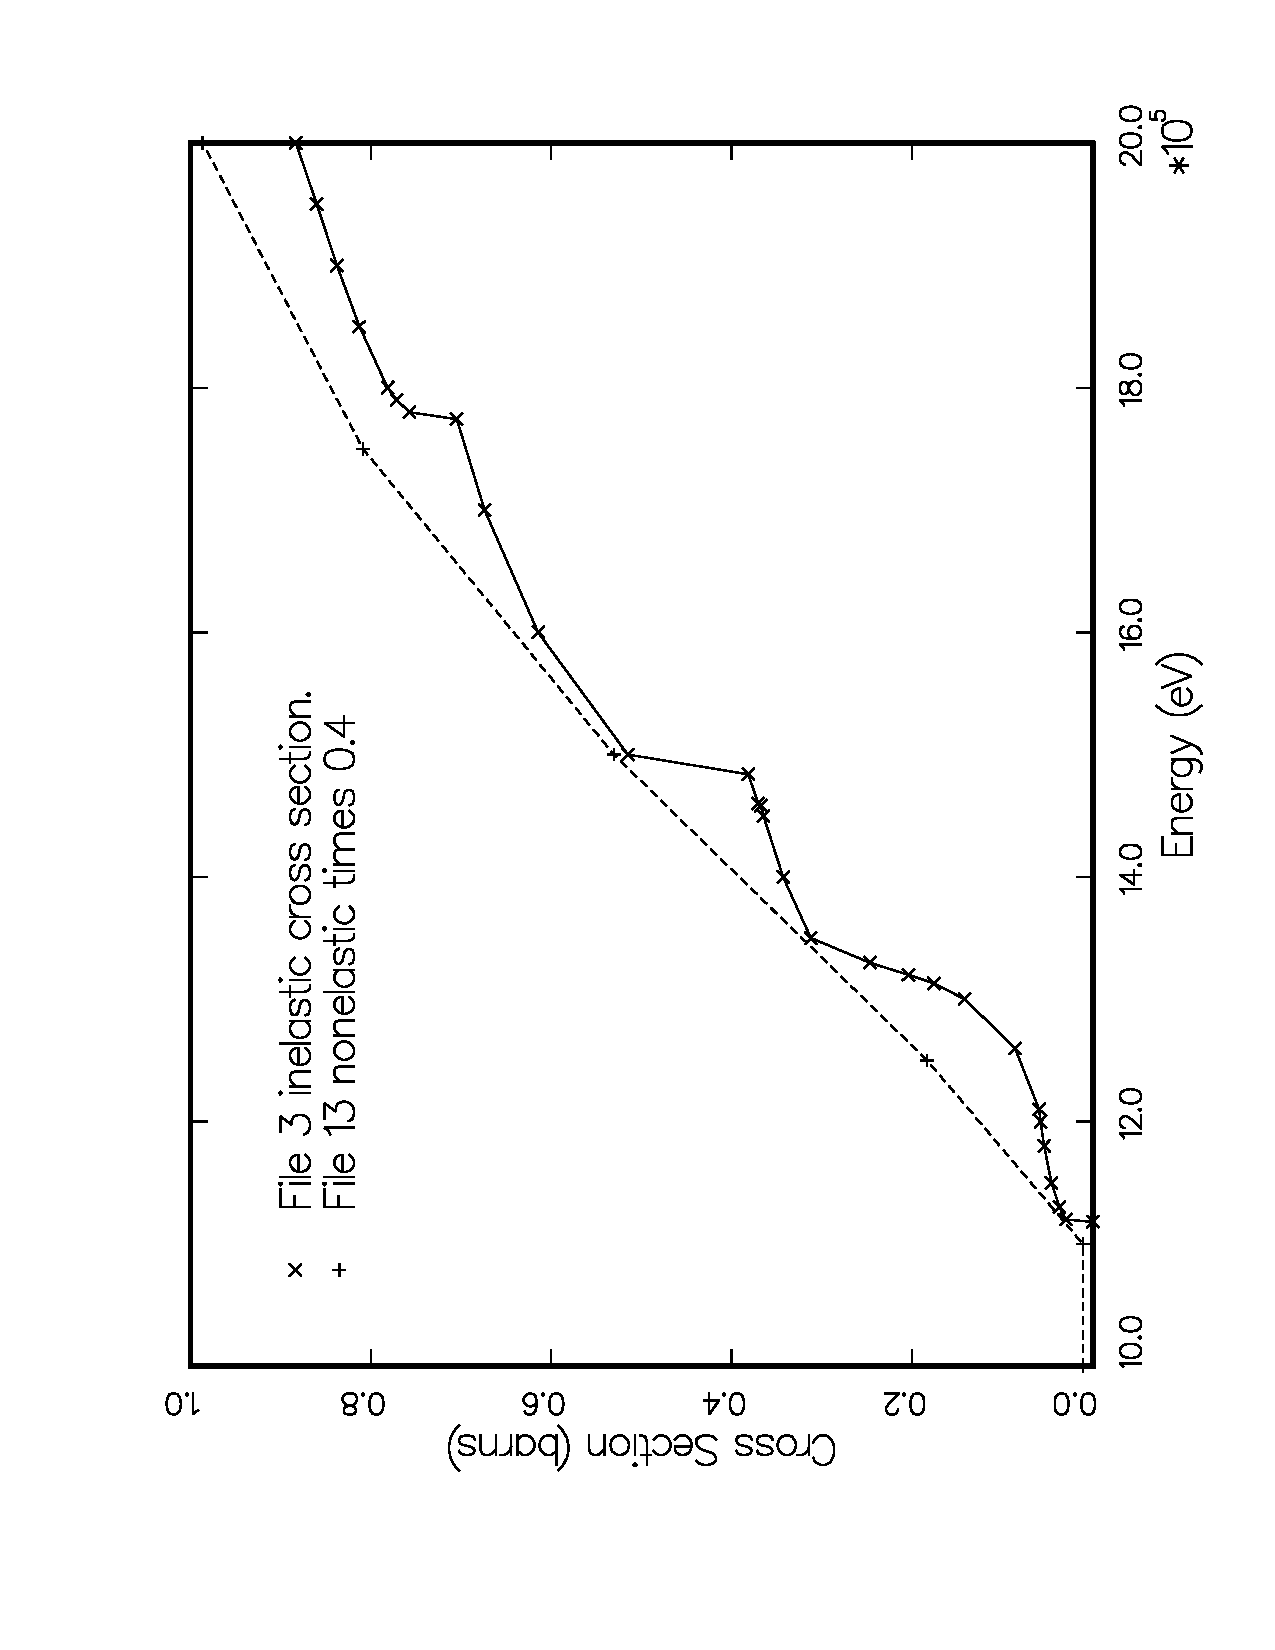
\includegraphics[keepaspectratio,height=3.2in, angle=270]{figs/heatr6ack}
\caption[Example of File 3 and File 13 energy grid mis-match]{Plot
 showing  the mismatch between the energy grids used for File 3
 and File 13 in the region of the thresholds for discrete-inelastic
 scattering levels for the case shown in Fig.~\ref{he5}. The cross
 and ex symbols show the actual grid energies in the evaluation.}
\label{he6}
\end{figure}

\begin{figure}[b]\centering
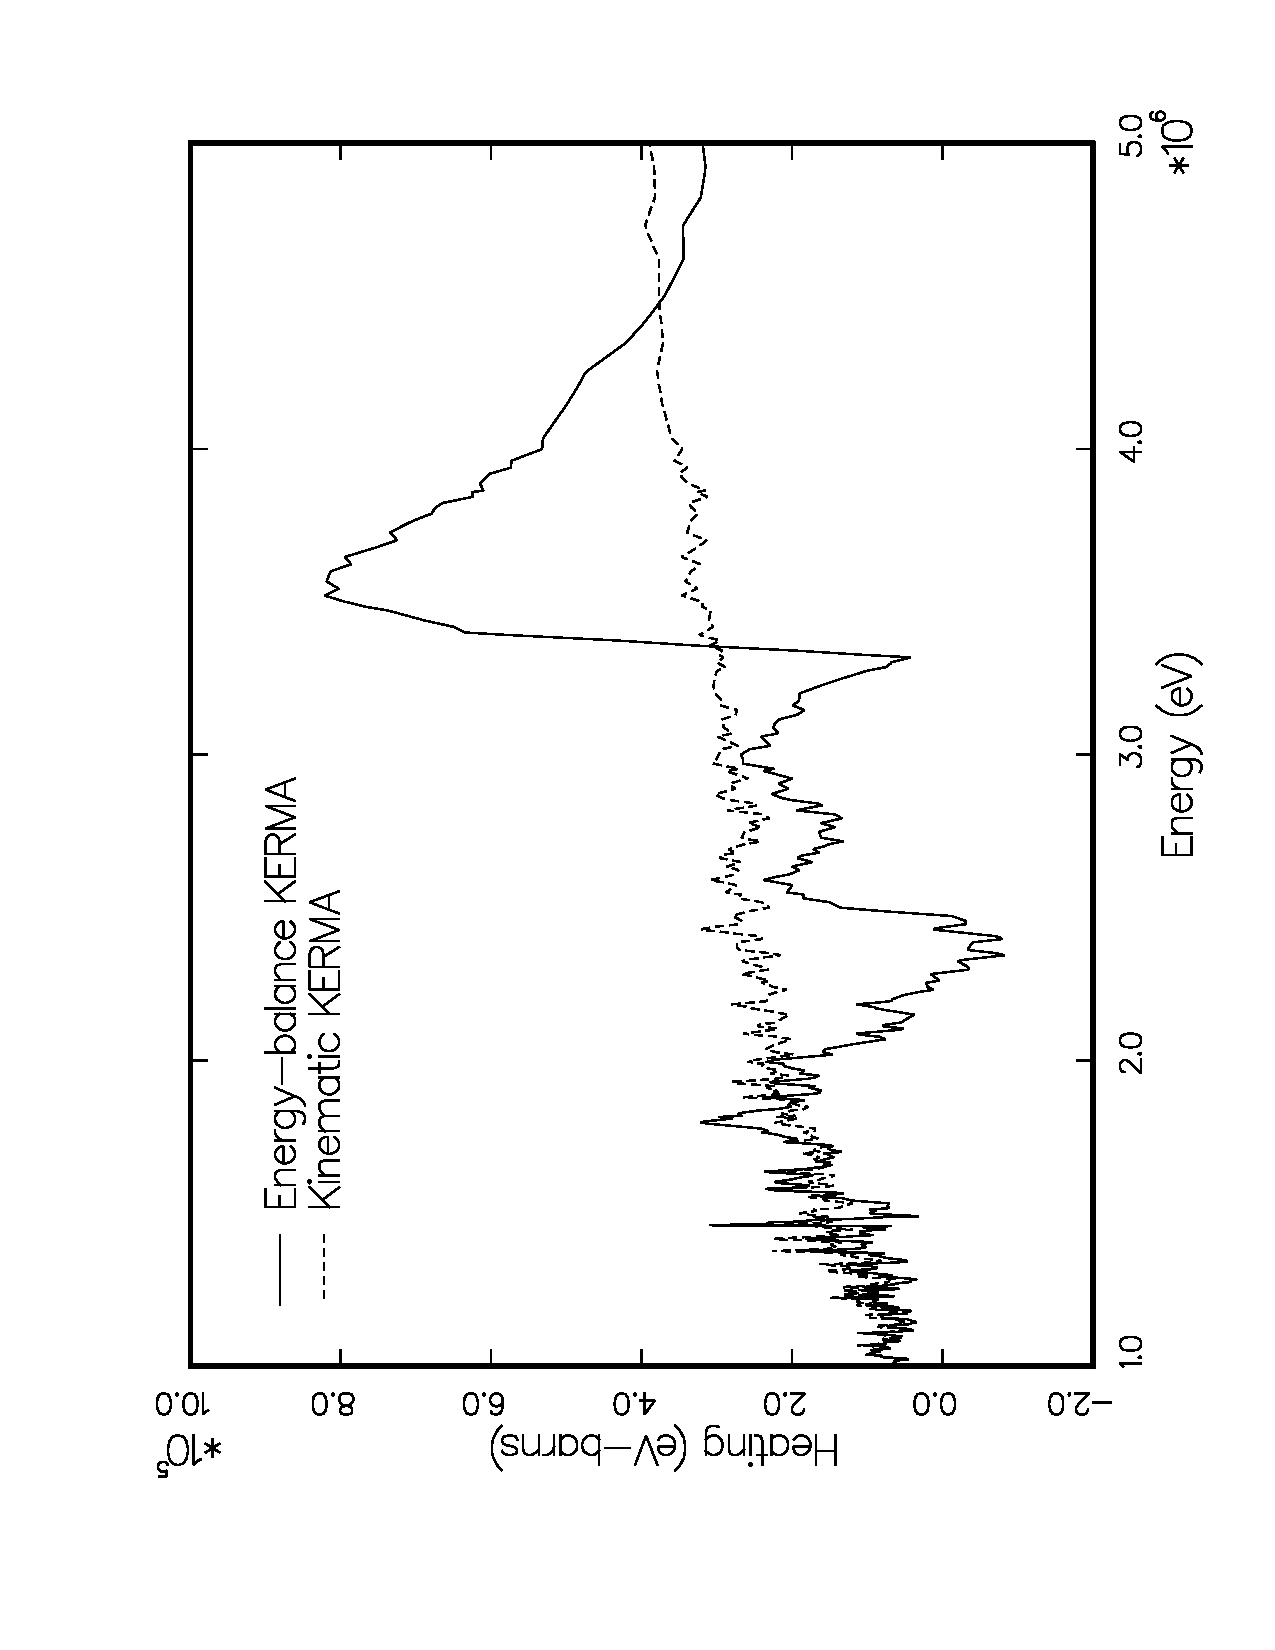
\includegraphics[keepaspectratio,height=3.2in, angle=-90]{figs/heatr7ack}
\caption[Example of energy-balance problems]{Typical energy-balance
 problems between points where balance is satisfied.  Discrete photons
 were used below about 2 MeV, and energy balance is reasonably good
 there.  The energy points in MF=13 for the continuum part are at 2, 3, and
 5 MeV, and the balance is also good at those energies.  Clearly, a grid
 in File 13 that used steps of about 0.25 MeV between 2 and 4 MeV would
 reduce the size of the deviations substantially and remove the negative
 KERMA factors.}
\label{he7}
\end{figure}

A method that is frequently used by evaluators of photon production
files is to select a number of nonelastic photon spectra on a
fairly coarse incident-energy grid using theory or experiment,
and then to readjust the photon yield on this energy grid so as
to conserve energy at each grid point.  However, the results do
not, in general, conserve energy at intermediate points.  If a
very coarse energy grid is used for File 13, quite large
deviations between MT=301 and MT=443 can result.  Fig.~\ref{he7}
shows such a case.  The solution to this kind of violation of
energy balance is to add intermediate points in Files 13 and 15
until the magnitude of the deviations is small enough for
practical calculations.

Especially large energy-balance errors of this type are caused
by interpolating across the minimum formed by the decreasing
capture heating and the increasing inelastic heating.
Fig.~\ref{he8} shows a dramatic example using a photon energy
production comparison.

\begin{figure}[bp]\centering
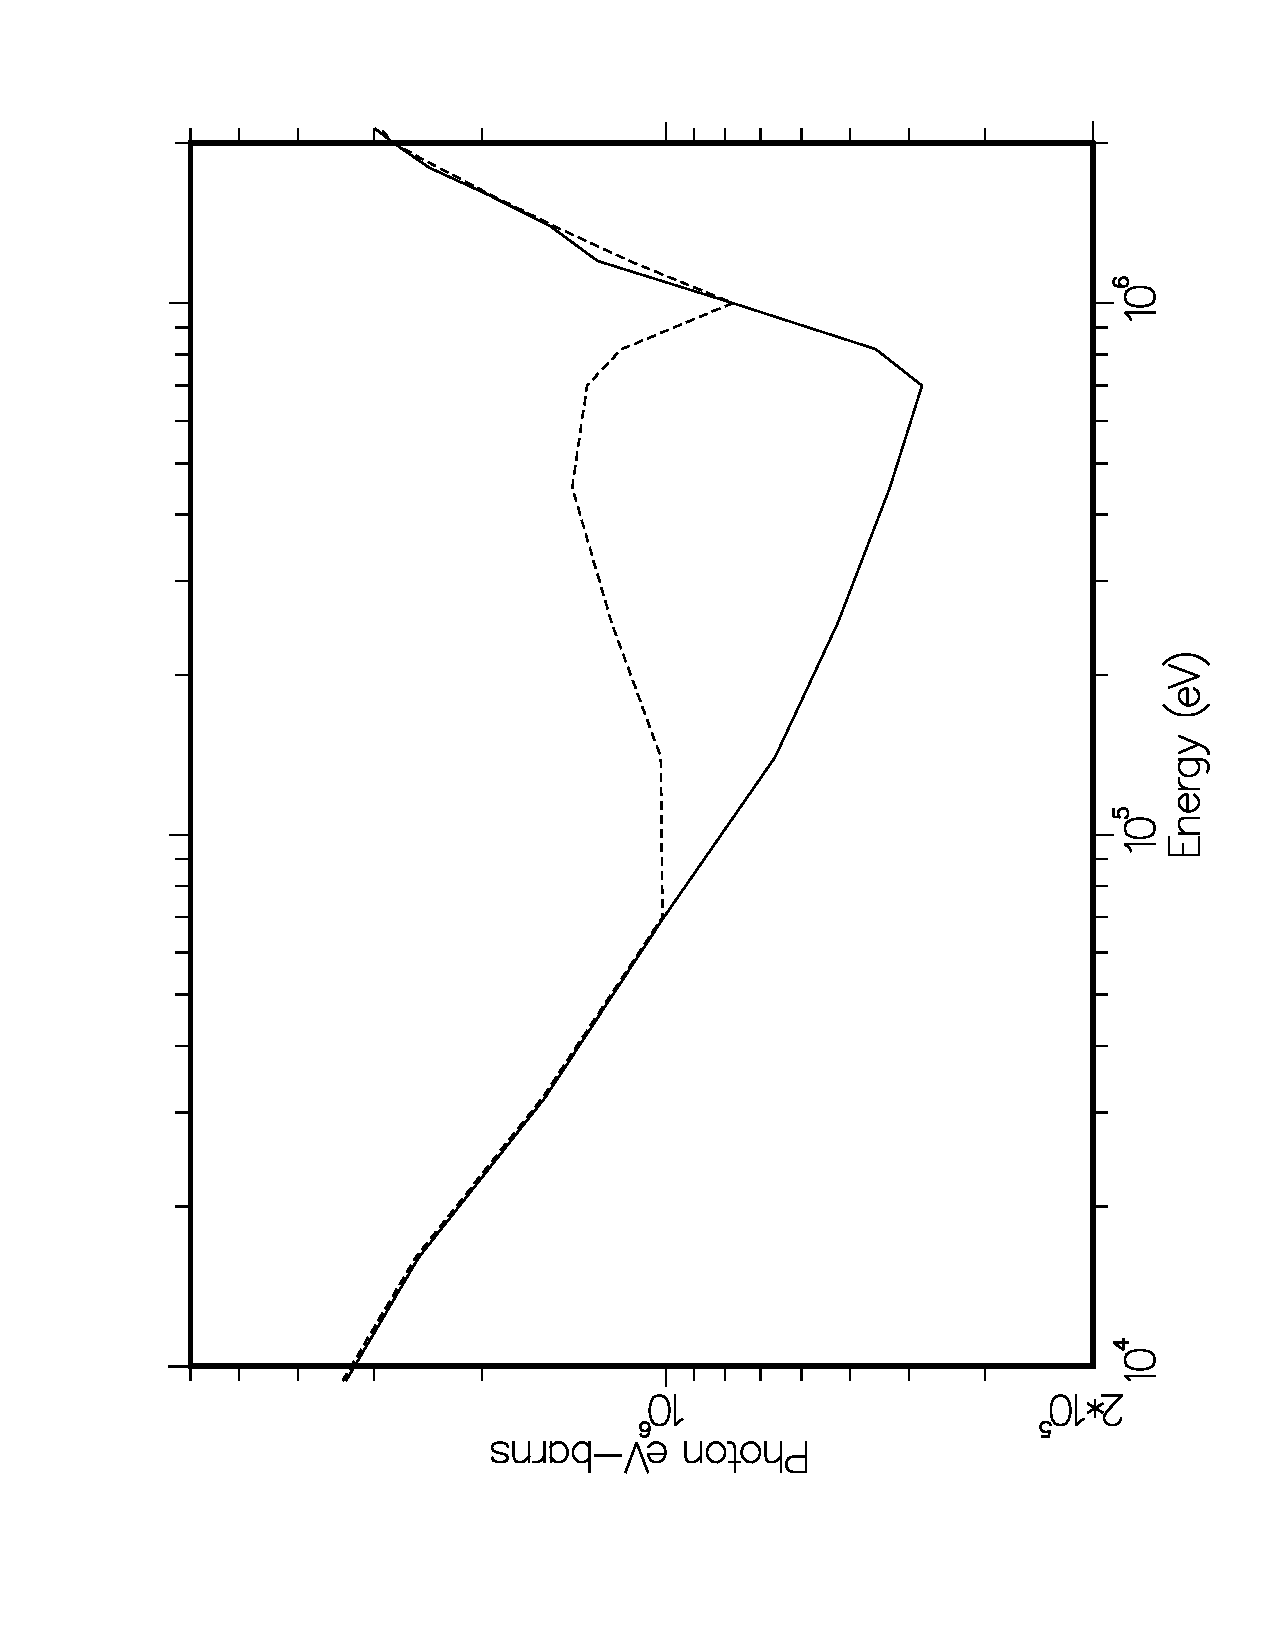
\includegraphics[keepaspectratio,height=3.5in, angle=270]{figs/heatr8ack}
\caption[Computed photon energy production and kinematic values]{Computed
 photon energy production (dashed) compared with the kinematic value
 (solid) for $^{93}$Nb from ENDF/B-V.  The original File 13 has grid points
 at 100 keV and 1 MeV.  Interpolating across that wide bin gives a photon
 production rate that is much too large for energies in the vicinity of a few
 hundred keV.  This will result in a large region of negative heating
 heating numbers.  Since this is just the region of the peak flux in a fast
 reactor, niobium-clad regions could be cooled instead of heated!}
\label{he8}
\end{figure}

For energies above the threshold for continuum reactions like
(n,n$'$) or (n,2n), it is difficult to use the results of the
kinematic checks to fix evaluations.  The representation of
Eqs.~\ref{contin} and \ref{contin2} for continuum inelastic
scattering is very rough.  Comparison to other more accurate
methods suggests that a CM formula would be better
here\cite{advanced}, even though the ENDF file says ``lab.''
Most other reactions give very wide low and high limits.  Two
exceptions are (n,2n) and (n,3n).  If they dominate the cross
section, the kinematic limits will be fairly close together.
In the 14 MeV range, energy errors could be in the photon data,
the neutron data, or both.  The best way to eliminate balance
errors is to construct a new evaluation based on up-to-date
nuclear model codes.

\subsection{Coding Details}
\label{ssHEATR_details}

The main subroutine is \cword{heatr}\index{heatr@{\ty heatr}}, which is
exported by module \cword{heatm}\index{modules!heatm@{\ty heatm}}.
It starts by reading the user's input and locating the desired
material on the PENDF\index{PENDF} file.  The main loop is over
temperature.  For each temperature, a check is made to see if
the user provided a value for the damage displacement energy.
If not, a default value is provided.  Next, \cword{hinit}
\index{hinit@{\ty hinit}} is called to examine the directory.  Flags
are set if MF=12 or 13 is present, if MT=18 or 19 is used, and if
MT=458 is present (see \cword{mgam}, \cword{mt19}, and \cword{mt458}).
The flags \cword{mt103}, \cword{mt104}, \cword{mt105}, \cword{mt106}
and \cword{mt107} are set if the corresponding particle production
levels are present.  The MT numbers used for the levels depend on
whether the input file used version 6 format or one of the earlier
formats.  For example, \cword{mt103} is set if MT=600-649 is found
for ENDF-6 data, or if MT=700-719 is found for earlier versions.
The code also checks to see if the corresponding angular distribution
data are present (see \cword{nmiss4}).  If any are not present, the
code will assume they are isotropic.  Note that \cword{hinit} also
collects a list of the File 6 MT numbers in \cword{mt6(i6)}.
For fissionable materials, the delayed fission energy values
are retrieved from MF=1/MT=458, and the correction, \cword{qdel}, is
computed for later use when calculating the heating from prompt
fission.

The next step in \cword{hinit} is to make a copy of File 6 on a
scratch file (if any sections of File 6 were found).  While doing
this, it searches through the subsections for each reaction
accumulating the ZA residual remaining after each particle is
given.  If it comes to the photons (\cword{zap}=0), which should
be last, and there is still a ZA residual left, then it concludes
that there is no subsection describing the residual.  It loads
a value into \cword{mt6no(ii6)} that is the index to the
subsection that the recoil should have followed had it been
present.  If it comes to the end of the subsection list without
finding photons and still has a ZA residual, it sets \cword{mt6no(ii6)}
to \cword{nk}; that is, the residual missing should follow the last
subsection.  In either case, the routine prints out messages
about ``photon recoil correction'' or ``one-particle recoil
approximation.''

Finally, \cword{hinit} makes a standardized copy of the ENDF tape
using \cword{hconvr}\index{hconvr@{\ty hconvr}}, and it also saves
the grid of the total cross section (MT=1) on the \cword{loada/finda}
scratch file that will be used to accumulate the KERMA factors,
damage, and kinematic checks (if requested).  Note also \cword{mt303},
which tells which of the requested edits is for nonelastic heating,
MT=303.  This is used later for writing out the photon energy
production check.

Now \cword{nheat}\index{nheat@{\ty nheat}} is called.   Its basic
function is to loop over the ``nonredundant'' reactions in File 3,
and to accumulate the corresponding contributions to the partial
heating and partial damage values into the appropriate elements
of the \cword{c} array on the \cword{loada/finda} file.  Redundant
reactions are reactions that duplicate or include effects that
can be obtained from another MT number.  They are determined using
a set of \cword{if} statements just after the entry to the reaction
loop at statement number 105.  The structure of the \cword{c} array
depends on whether kinematic checks are being accumulated or not
and whether photon production files are present.  If neither
occurs, the structure has \cword{npk}+1 elements as follows:

\begin{center}
\begin{tabular}{cl}
Element & Contents \\ \hline
\cword{1} & energy \\
\cword{2} & total heating \\
\cword{3} & value for first partial \\
$\cdots$ & \\
\cword{npk}+1 & value for last partial \\ \hline
\end{tabular}
\end{center}

\noindent
where \cword{npk} is the number of partial KERMA or damage
values being accumulated, including the total.
If checks are being accumulated, the \cword{c} array has the
following 3*\cword{npk}+1 elements:

\begin{center}
\begin{tabular}{cl}
Element & Contents \\ \hline
\cword{1} & energy \\
\cword{2} & total heating \\
\cword{3} & value for first partial \\
$\cdots$ & \\
2+\cword{npk} & lower kinematic limit for total \\
3+\cword{npk} & lower kinematic limit for first partial \\
$\cdots$ & \\
2+2*\cword{npk} & upper kinematic limit for total \\
3+2*\cword{npk} & upper kinematic limit for first partial \\
$\cdots$ & \\
3*\cword{npk}+1 & upper kinematic limit for last partial \\ \hline
\end{tabular}
\end{center}

\noindent
If photon production files are present in the evaluation, the total
length of the \cword{c} array increases by the following three
words (\cword{len} is the old length from above plus three):

\begin{center}
\begin{tabular}{cl}
Element & Contents \\ \hline
\cword{len}-2 & photon capture correction \\
\cword{len}-1 & total photon eV-barns \\
\cword{len} & total energy yield for ``subtot'' \\ \hline
\end{tabular}
\end{center}

Back inside the loop over nonredundant reactions, subroutine
\cword{gety1}\index{gety1@{\ty gety1}} is initialized for this
reaction.  The code checks to see if this section uses File 6
for its distributions; if so, it arranges to make multiple passes
through the reaction's energy grid, one pass for each subsection
of the MF=6 section, and perhaps one additional pass to synthesize
the missing recoil subsection.  It is now possible to select the
appropriate $Q$-value and particle yield, and to initialize the
appropriate calculational routine.  This routine will be
\cword{sixbar}\index{sixbar@{\ty sixbar}} for all reactions
described in File 6, \cword{disbar}\index{disbar@{\ty disbar}} for
two-body reactions using File 4 (including charged-particle
reactions in the 600 or 700 series of MT numbers),
\cword{conbar}\index{conbar@{\ty conbar}} for continuum reactions
represented using File 5, and \cword{capdam}\index{capdam@{\ty capdam}}
for the neutron disappearance reactions (MT=102, 103, {\it etc.})
and the charged-particle continuum reactions from the 600 or 700
series of MT numbers.  The last step before beginning the energy
loop for this reaction is to call \cword{indx}\index{indx@{\ty indx}},
which determines which element of the \cword{c} array is to receive
the heating or damage contribution from this reaction (see below).

The energy loop in \cword{nheat}\index{nheat@{\ty nheat}} goes
through statement number 190.  For each energy,
\cword{finda}\index{finda@{\ty finda}} is called to retrieve the current
values for the energy [see \cword{c(1)}] and the partial heating
and damage values as accumulated so far.  On the first pass
through the scratch file, the list of energies to be used for
printing information on the listing is established in
\cword{elist} using a few \cword{if} statements based on the
range of the energy variable \cword{e}.  For each energy, the
corresponding cross section is retrieved using
\cword{gety1}\index{gety1@{\ty gety1}} and
the appropriate $\overline{E}$ and damage numbers are computed
by calling \cword{getsix}\index{getsix@{\ty getsix}},
\cword{disbar}\index{disbar@{\ty disbar}},
\cword{conbar}\index{conbar@{\ty conbar}}, or
\cword{capdam}\index{capdam@{\ty capdam}}.  The heating contribution
is computed from the appropriate formula, and the heating and damage
numbers are summed into the \cword{c} array at location \cword{index}.
If requested, the kinematic limits on the heating are computed and
summed into the \cword{c} array at \cword{index}+\cword{npk} and
\cword{index}+2*\cword{npk}.  The completed results for this energy and
reaction are written out onto the \cword{loada/finda} scratch file,
and the energy loop is continued.

When the energy loop is complete, the subroutine jumps to the
next section (or subsection in the case of File 6) and repeats the
entire energy loop for that reaction (or particle from File 6).

Subroutine \cword{indx}\index{indx@{\ty indx}} is used to
select what element of the \cword{c} array is to receive the
heating or damage contribution for a section with a particular
MT number.  The meaning of each element of the \cword{c} array
is obtained from the \cword{mtp} array.  Normally, a reaction
MT contributes to the partial heating element with
\cword{mtp(i)}=MT+300.  But it can also contribute to
several other elements of \cword{c}, such as nonelastic
(MT=303), inelastic (MT=304), etc.  Therefore, \cword{indx}
returns the count of reactions contributed to by \cword{mt}
in \cword{nmt} and the indexes for the \cword{c} array in
\cword{imt(nmt)}.

Subroutine \cword{capdam}\index{capdam@{\ty capdam}}
is used to compute the damage energy for neutron capture
(or disappearance) reactions; that is, for MT=102, 103,
etc.  On the initialization entry (\cword{ee}=0.0), the
routine sets up various kinematics parameters, such as \cword{zx}
and \cword{ax} to describe the outgoing particle, and initializes
\cword{df}.  In order to save time, the routine only calculates the
damage on a grid that increases by steps of 10\%.  Intermediate
values are obtained by interpolation (see \cword{el}, \cword{daml},
\cword{en}, and \cword{damn}).  The values at the grid points
are computed using

\begin{equation}
   D\left(\frac{E}{A+1}\right)
    +D\left(\frac{1}{2M_Rc^2}\left[\frac{AE}{A+1}+Q\right]^2\right)
\end{equation}

\noindent
for radiative capture (the corrections for multiple photon emission
will be made later), or using Eq.~\ref{damint} with $E_R$
from Eq.~\ref{npart} and a 4-point Gauss-Legendre
\index{Gauss-Legendre quadrature} quadrature.  The angular
distribution for particle emission is taken to be isotropic.

Subroutine \cword{disbar}\index{disbar@{\ty disbar}} is used by
\cword{nheat} to compute the average secondary energy and damage
energy for elastic scattering (MT=2), discrete-inelastic scattering
(MT=51-90), or discrete-level particle production (MT=600-648,
650-698, etc. for ENDF/B-VI or ENDF/B-VII, or MT=700-717,
720-737, etc. for earlier versions).  It starts by initializing
\cword{hgtfle}\index{hgtfle@{\ty hgtfle}} (which is very similar to
\cword{getfle}\index{getfle@{\ty getfle}} in the GROUPR module),
determining kinematic parameters like \cword{awp} (the mass ratio
to the neutron for the emitted particle), and initializing
\cword{df}\index{df@{\ty df}}.  In order to save time, it only
computes the heating and damage on a grid based on steps by a
factor of 1.1 and the \cword{enext} values from \cword{hgtfle}.
On a normal entry, it interpolates between these values (see
\cword{el}, \cword{cl}, \cword{daml}, \cword{en}, \cword{cn}, and
\cword{damn}).  When the desired \cword{ee} exceeds \cword{en},
the old high values are moved down to the low positions, and new
high values are calculated.  The calculation of \cword{cn}
follows Eq.~\ref{enb}.  The calculation of \cword{damn} uses
Eq.~\ref{damint} with a 20-point Gauss-Legendre quadrature
(see \cword{nq}, \cword{qp}, and \cword{qw}).

Function \cword{df}\index{df@{\ty df}} is used to compute the
damage partition function given in Eq.~\ref{robinson}.  The
constants that depend on the recoil atom or particle type and
lattice type (see \cword{zr}, \cword{ar}, \cword{zl}, \cword{al})
are computed in an initialization call with \cword{e}=0.0.  Thereafter,
it can be called with any other value of \cword{e}.

Similarly, \cword{conbar}\index{conbar@{\ty conbar}} computes
the average secondary energy and damage energy for continuous
distributions described in File 5.  Analytic representations use
simple formulas coded into \cword{anabar}\index{anabar@{\ty anabar}}
or a combination of adaptive and Gaussian quadrature in
\cword{anadam}\index{anadam@{\ty anadam}}.  Tabulated data are
interpolated from the File 5 table using
\cword{tabbar}\index{tabbar@{\ty tabbar}} or integrated using
trapezoidal and Gaussian quadratures in
\cword{tabdam}\index{tabdam@{\ty tabdam}}.  As usual, the routine
is initialized by calling it with \cword{e}=0.0.  The
secondary-particle yield is either chosen from the MT number,
or \cword{hgtyld}\index{hgtyld@{\ty hgtyld}} is initialized.  The
desired section of File 5 is located on the input ENDF tape, and the
kinematic constants are computed.  The reactions
with MT=22, 28, 32, 33, and 34 will be treated using the
\cword{capdam}\index{capdam@{\ty capdam}} method; if
\cword{mtd} has one of these values (see \cword{mtt}),
\cword{capdam} is initialized.  As is the case for
\cword{getsed}\index{getsed@{\ty getsed}} in the
\hyperlink{sGROUPRhy}{GROUPR}\index{GROUPR}
module, this routine can handle some sections of File 5 that contain
multiple subsections, but the analytic subsections must come
first.  As each analytic subsection is read, appropriate data
are stored in in the external array \cword{c} using pointers
saved in the array \cword{loc}.  Only the first energy is read
and stored for a tabulated subsection (\cword{lf}=1).  The
idea is to have only two energy values in memory at a time
in order to save storage; the second subsection will be read
during the first normal entry to the subroutine.  The final
step in the initialization pass is to initialize
\cword{df}\index{df@{\ty df}}.  For a normal entry into
\cword{conbar}\index{conbar@{\ty conbar}}, the energy-dependent
fission yield is retrieved, if needed, and the loop over
subsections is entered.  Each subsection in File 5 starts
with a fractional-probability record.  The desired value
for energy \cword{e} is computed by interpolation using the
standard \hyperlink{sNJOYhy}{NJOY} utility routine
\cword{terpa}\index{terpa@{\ty terpa}}.
For analytic subsections, the routine uses
\cword{anabar}\index{anabar@{\ty anabar}} to compute
$\overline{E_n}$, and \cword{anadam} or
\cword{capdam}\index{capdam@{\ty capdam}} to
compute the damage energy. Note that in order to save time,
\cword{anadam} is only calculated on a fairly coarse grid
based on steps by a factor of 1.5.  The intermediate values
are obtained by interpolation using
\cword{terp1}\index{terp1@{\ty terp1}}.  For
tabulated subsections, \cword{ebar} and \cword{dame} values
are normally obtained by interpolation (see \cword{elo},
\cword{flo}, \cword{dlo}, \cword{ehi}, \cword{fhi}, and
\cword{dhi}).  However, for the first entry, or whenever
\cword{e} reaches \cword{ehi}, the high data are moved into
the low positions, new high data are read from the File 5
subsection, and the values for heating and damage
are computed at \cword{ehi} using
\cword{tabbar}\index{tabbar@{\ty tabbar}} and
either \cword{tabdam}\index{tabdam@{\ty tabdam}} or
\cword{capdam}\index{capdam@{\ty capdam}}.

Subroutine \cword{hgtyld}\index{hgtyld@{\ty hgtyld}} is
similar to \cword{getyld}\index{getyld@{\ty getyld}} in the
\hyperlink{sGROUPRhy}{GROUPR}\index{GROUPR}
module.  It finds the required section on
the ENDF tape and reads the entire LIST or TAB1 record into
memory.  On normal entries, it either computes the yield using the
polynomial formula with constants from the LIST record, or
it uses \cword{terpa}\index{terpa@{\ty terpa}} to interpolate for
the yield in the TAB1 data.

Subroutine \cword{anabar}\index{anabar@{\ty anabar}}
is used to compute the average energy for a neutron described
by an analytic subsection of File 5.  The simple formulas
used are tabulated in the ENDF format manual\cite{ENDF102}.
Similarly, \cword{anadam}\index{anadam@{\ty anadam}} is used to
compute the damage energy for an analytic subsection of File 5.
Only LF=9 (the Simple Maxwellian Distribution) is supported; the
routine returns zero for other laws.  Note that a statement function
is defined to compute the secondary energy distribution for
this law (see \cword{sed}).  For each incident energy, the
spectrum temperature \cword{theta} is retrieved using
\cword{terpa}, and an adaptive integration stack is
initialized with points at four secondary energies,
namely, 1., $.5(E{-}U)$, $\theta$, and $E{-}U$, where $U$ is
a parameter that sets the maximum possible value of $E'$.
The adaptive procedure proceeds to solve Eq.~\ref{f5dam}
by subdividing this starting grid until trapezoidal integration
can be used on each panel.  The inner integral over emission
cosine $\mu$ is performed using a 4-point Gauss-Legendre
quadrature for each point on the adaptive grid.  The
function \cword{sed} is used to compute $g(E')$, and
\cword{df}\index{df@{\ty df}} is used to compute the
partition function.

Subroutine \cword{tabbar}\index{tabbar@{\ty tabbar}}
is used to compute the average energy of the emitted neutron
for a tabulated subsection of File 5.  It can also be used
for a tabulated subsection of File 6.  This option is
flagged by \cword{law} negative.  The trick is to set
the ``stride'' or ``cycle'' through the file to be larger
than 2 (see \cword{ncyc}).  The angular part of the
$g(E{\rightarrow}E')$ table is skipped, and only the $E'$ and
$g$ values are retrieved.  For File 5, this routine only works
for laws 1 and 5; others cause a fatal error message to be
issued.  In both of these cases, the integral over $E'$ needed
to compute the average energy is done analytically for each
panel in the input data using a different formula for each
interpolation scheme \cword{int}.

Subroutine \cword{tabdam}\index{tabdam@{\ty tabdam}}
is used to compute the damage energy for a tabulated subsection
of File 5.  The integration that is needed is given in
Eq.~\ref{f5dam}.  The energy grid of the tabulation
is assumed to be good enough to allow trapezoidal
integration to be used for $E'$, and a 4-point Gauss-Legendre
quadrature is used for $\mu$.

Subroutine \cword{sixbar}\index{sixbar@{\ty sixbar}}
is used to compute charged-particle average energy and
damage energy represented by using a subsection of File 6.
As is common with NJOY subroutines, \cword{sixbar} is
initialized by calling it with \cword{e}=0.0.  The initialization
path is controlled by \cword{j6}, which is the index
to the current subsection in File 6; by \cword{irec},
which is 1 when a recoil response is to be calculated, and
by \cword{jrec}, which tells the routine how to get back to
the next subsection after a recoil calculation.  If this is
not a recoil subsection, the routine jumps to statement 110
and starts reading in the data for the desired subsection.
If it is flagged as a recoil (see \cword{irec}), the routine
backs up to the subsection describing the particle that induced
the recoil and then continues by reading in the data for that
particle.

The first step is to read in the TAB1 record
that contains the particle yield, identity (\cword{zap}
and \cword{awp}), and representation \cword{law}.
If this law describes a two-body recoil distribution, the
routine sets \cword{jrec} for a proper return, sets
\cword{irec} to back up to the corresponding direct emission
subsection, and jumps back to the beginning of the routine
to do the recoil calculation.

When the code finally arrives at statement number 210, it is
ready to start processing the current subsection.  It reads
in the parameters for laws 3 and 6, or the TAB2 record and
the data for the first energy point for the other laws.  With
the data in place, it computes the corresponding values
for mean energy and damage energy using
\cword{getsix}\index{getsix@{\ty getsix}} or
\cword{tabsq6}\index{tbsq6@{\ty tabsq6}} and returns.

In the special case where the section contains only a single
subsection that describes a neutron, the data stored in
memory will be the data for that subsection, and the
subroutine \cword{tabbar}\index{tabbar@{\ty tabbar}} with a
negative value for the law is used to produce the low values.

On a normal entry (\cword{e}$>$0),
\cword{sixbar}\index{sixbar@{\ty sixbar}} checks to
see whether \cword{e} is in the current interpolation range.
If it is, the code jumps to statement number 400.  For the
analytic laws (\cword{law}=3 and \cword{law}=6), it uses
a direct call to \cword{getsix} to compute the mean energy
and damage energy.  For the tabulated laws, it interpolates
for the results using the low and high data (see \cword{elo},
\cword{flo}, \cword{dlo}, \cword{ehi}, \cword{fhi}, and
\cword{dhi}).  On the first entry, or whenever \cword{e}
increases to \cword{ehi}, the code moves the high data to
the low positions, and then it reads in the data for the
next energy and computes a new set of high values for
mean energy and damage using \cword{getsix} or \cword{tabsq6}.

Subroutine \cword{getsix}\index{getsix@{\ty getsix}}
is used to compute the mean energy and damage energy for
one particular incident energy in a subsection of File 6.
The method used depends on the value of \cword{law} and
the reference frame for the subsection.  The first case
in the coding is for \cword{law}=1 with data in the CM system.

This case uses Eqs.~\ref{KofE} and \ref{DofE} with an
adaptive integration over $E'$.  The integration stack is
contained in the arrays \cword{x} and \cword{y}.  It is
primed with \cword{x(2)}=0, and \cword{h6cm} is called to
compute \cword{y(2)} and the next grid point \cword{epnext}.
The first panel is completed by calculating \cword{y(1)} and
\cword{x(1)}=\cword{epnext}.  The panel is then divided in half, and
the midpoint is tested to see if it is within \cword{tol}=0.02
({\it i.e.}, 2\%) of the linearly interpolated value.  If
not, the midpoint is inserted in \cword{x} and \cword{y},
and the new top panel [that is \cword{x(2)}$-$\cword{x(3)}]
is tested.  This continues until convergence is achieved in
the top panel.  The contributions to the heating and damage
are added into the accumulating integrals at statement
number 190, and \cword{i} is decremented so that the process
can be repeated for the next panel down.  When \cword{i}
decreases to one, the current value of \cword{epnext} is
used to start the next higher $E'$ panel.  This loop over
panels continues until the entire $E'$ range has been
integrated.

The next special case is for tabulated distributions that use
$E$, $E'$, $\mu$ ordering in the lab system.  The angular part
is ignored.  A simple loop over the \cword{NEP} points in
$g(E{\rightarrow}E')$ is carried out.  Trapezoidal integration
is used for each panel for both heating and damage (\cword{h}
and \cword{d}).  If \cword{nd}$>$0, the first \cword{nd} entries
are discrete energies, and the values of the integrand at
those energies are added into \cword{h} and \cword{d}.
Finally, \cword{h} and \cword{d} are copied into \cword{ebar}
and \cword{dame}.

The block of coding starting at statement number 450 is used to
compute particle mean energies for the emitted particles from
two-body reactions, or to compute the mean recoil energy for a
two-body reaction (see \cword{irec}$>$0).  The calculation
follows Eq.~\ref{ebar6}.  Note that the kinematic factors
include \cword{awp}, the mass ratio of the emitted particle to
the incident particle.  The parameter \cword{beta} here is
the same as $R$ in Eq.~\ref{beta}.  If the angular
distribution in File 6 is in Legendre form, the heating
and damage integrals are performed using a 20-point
Gauss-Legendre quadrature (see \cword{nq}, \cword{qp},
and \cword{qw}).  If the angular distribution is tabulated
as $f(\mu)$ {\it versus} $\mu$, a trapezoidal integration is used
for both heating and damage.

The final option in \cword{getsix} is for lab distributions
that use $E$, $\mu$, $E'$ ordering.  See Eq.~\ref{llnl}.
The inner integrals are computed using trapezoidal integration.
The outer integral over $\mu$ also uses trapezoidal integration
on the results of the inner integrals for each $\mu$ grid point.

Note that \cword{getsix} has an \cword{irec} parameter in its
calling list.  When this parameter is greater than zero, the
angular distribution is complemented and the charge and mass of
the particle are modified to represent the recoil species.
The value of \cword{irec} is controlled by \cword{sixbar}.

Subroutine \cword{h6cm}\index{h6cm@{\ty h6cm}} is used by
\cword{getsix} to compute the lab distribution
$g(E{\rightarrow}E'_L)$ of Eq.~\ref{transCM}
using the CM data in File 6.  This subroutine uses
\cword{h6dis}\index{h6dis@{\ty h6dis}},
\cword{h6ddx}\index{h6ddx@{\ty h6ddx}} and
\cword{h6psp}\index{h6psp@{\ty h6psp}} to retrieve the CM discrete,
tabulated or phase-space data from the file.  These routines are
basically the same as \cword{f6cm}\index{f6cm@{\ty f6cm}},
\cword{f6dis}\index{f6dis@{\ty f6dis}},
\cword{f6ddx}\index{f6ddx@{\ty f6ddx}}
and \cword{f6psp}\index{f6psp@{\ty f6psp}}.  See
\hyperlink{sGROUPRhy}{GROUPR}\index{GROUPR} for more details.

Subroutine \cword{gheat}\index{gheat@{\ty gheat}}
is used to correct the heating and damage values accumulated
during the pass through the neutron sections.  It loops through
all of the reactions in File 12 and File 13 using two
ENDF-type tapes.  One is the input PENDF tape, which is used
to retrieve cross sections for use with the photon
multiplicities in File 12.  The other is a version of
the input ENDF tape that has been passed through
\cword{hconvr}\index{hconvr@{\ty hconvr}} to put the photon
data in a standard form (see
Chapter \ref{sGROUPR} (\hyperlink{sGROUPRhy}{GROUPR})
\index{GROUPR} of this manual for a more detailed
discussion of \cword{conver}\index{conver@{\ty conver}}).
This scratch tape is used to retrieve the File 12 and File 13
data.  It is very common to find reaction MT=3 (nonelastic)
in File 12, but this reaction has been removed from the PENDF
tape because it is redundant; that is, it is equal to MT1$-$MT2.
 Therefore, two passes are made through the File 12 data for
MT=3, an addition pass with MT=1 from the PENDF tape, and
a subtraction pass with MT=2 from the PENDF tape.  Once the
desired sections on the two tapes have been found, the subroutines
\cword{gambar}\index{gambar@{\ty gambar}},
\cword{capdam}\index{capdam@{\ty capdam}},
and \cword{disgam}\index{disgam@{\ty disgam}} are initialized.

The energy loop for \cword{gheat} goes through statement
number 190.  For each energy, \cword{finda}\index{finda@{\ty finda}}
is used to retrieve the partial KERMA factors as computed from the
pass through the neutron files.  The yield or cross section is
retrieved using \cword{gety1}\index{gety1@{\ty gety1}} into the
variable \cword{y}.  If necessary, the corresponding cross section
\cword{x} is retrieved using \cword{gety2}\index{gety2@{\ty gety2}}.
For cases where an
energy-dependent Q is available, it is retrieved using
\cword{terp1}\index{terp1@{\ty terp1}} on the data stored at
\cword{lqx}.  The next two lines correct the energy of ``primary''
photons (\cword{lp}=2).

For radiative capture represented in File 12 (MT=102),
\cword{gambar}\index{gambar@{\ty gambar}},
\cword{disgam}\index{disgam@{\ty disgam}}, and/or
\cword{capdam}\index{capdam@{\ty capdam}} are
called to return $\overline{E}_\gamma$ and
$\overline{E^2_\gamma}/(2m_Rc^2)$ for this photon spectrum
or discrete photon and to correct the heating and values
in the \cword{c} array using Eq.~\ref{cfix} and the second
line of Eq.~\ref{D102}.  The capture contribution to the
total photon eV-barns is added into \cword{c(npkk-1)} and
the photon energy yield is loaded into \cword{c(npkk)} for
each subsection.  When the last subsection is reached, the
capture energy check is made using this subtotal.  Note
that the capture error is loaded into \cword{c(npkk-2)}
for later use in calculating the kinematic limits for
photon energy production.

For other photon-production reactions, the photon eV-barns
contribution is subtracted from the energy-balance heating
position, added into the total photon energy value in
\cword{c(npkk-1)}, and added into \cword{c(npkk)} for the
subtotal for a section with multiple subsections.  After
all the corrections have been completed for this energy,
the revised values are written out using \cword{loada}.  The
code then moves on to the next reaction and repeats the
entire process.

When the reaction loop has been finished, \cword{gheat}
checks to see if it can print out a photon energy production
check.  It can do this if kinematic checks have been requested
and if MT=303 was requested in the user's list of partial KERMA
calculations.  The code reads through the \cword{loada/finda}
file one more time.  For each energy in \cword{elist}, it
prints out the total photon eV-barns from \cword{c(npkk-1)}
and the kinematic limits \cword{elo} and \cword{ehi}.  If the
limits are violated by more than 10\%, alarms consisting of the
strings \cword{++++} or \cword{----} are printed after the
eV-barns values.

Subroutine \cword{gambar}\index{gambar@{\ty gambar}}
is used to compute the mean energy for continuous photon
spectra and the photon recoil correction for capture.
When called with \cword{e}=0.0, it locates the
desired section of File 15 on the ENDF tape and reads in
the first incident energy.  On a normal entry, it checks to
see if \cword{e} is in the range of the data already computed
(\cword{elo}, \cword{ehi}, etc.), and if so, it interpolates
for the desired results.  If not (or on the first real entry),
it moves the high data down to the low positions, reads in the
next energy from File 15, prepares new values at the new
\cword{ehi}, and checks the energy range again.  The
photon \cword{ebar} is returned by \cword{tabbar}, and the
corrections to the heating value (\cword{esqb}) and damage
value (\cword{esqd}) from photon production are generated
using \cword{tabsqr}.

Subroutine \cword{tabsqr}\index{tabsqr@{\ty tabsqr}}
is used to compute the average recoil energy

\begin{equation}
   \frac{\overline{E_\gamma^2}}{2M_Rc^2}
\end{equation}

\noindent
for radiative capture for a tabulated subsection of File 15.
The corresponding damage energy is computed at the same time.
The basic secondary-energy integral is over the panels
defined by the grid points given in File 15.  Inside each
panel, the integral is computed using a 4-point Gauss-Legendre
quadrature.

Subroutine \cword{disgam}\index{disgam@{\ty disgam}}
is used to compute the $\overline{E_\gamma^2}$ and corresponding
damage energy for a discrete capture photon.  The rest-mass
constant is computed by calling \cword{disgam} once with \cword{e}=0.

Subroutine \cword{hout}\index{hout@{\ty hout}}
writes the new PENDF tape with the desired heating and damage
MT numbers added.  It also corrects the directory in MF=1/MT=451,
and it prepares the output listing for printing.  The first step
is to loop through the partial KERMA factors requested and to write
the data on the \cword{loada/finda} file onto a scratch tape
in ENDF File 3 format.  While the first partial is being
prepared, the code matches energies in \cword{c(1)} against
the energy list for printing in \cword{elist}.  When a match
is found, the partial KERMA factors are checked against the
kinematic limits, and the variables \cword{klo} or
\cword{khi} are set if any of the comparisons are out of
bounds.  The KERMA factors, kinematic limits, and error
flags are then printed on the output listing.  When all of
the new sections for File 3 have been prepared, the code
updates the contents of the File 1 directory.  It then
loops through the rest of the input PENDF tapes copying
sections to the output and inserting the new sections in
the appropriate places.  When the new PENDF file has been
completed, \cword{hout} makes \hyperlink{sVIEWRhy}{VIEWR}
\index{VIEWR} input for a set of
plots showing the total heating and the photon production
compared to their kinematic limits in both lin-lin and
log-log forms.  The lin-lin plots show the high-energy range
better, and the log-log plots expand the low-energy range.

\subsection{Error Messages}
\label{ssHEATR_msg}

\begin{description}
\begin{singlespace}

\item[\cword{error in heatr***requested too many kerma mts}] ~\par
  6 values in addition to MT=301 are allowed with kinematic checks;
  otherwise, 25 can be requested.  See \cword{npkmax}=28.  When
  checks are requested, the number of words needed is
  3*\cword{npk}+7; otherwise, \cword{npk}+3 are needed.

\item[\cword{error in heatr***requested too many q values}] ~\par
  Limited to 30 by the global parameter \cword{nqamax}=30.

\item[\cword{error in heatr***too much energy-dependent q data}] ~\par
  Limited to \cword{maxqbar}=10000.

\item[\cword{error in heatr***mode conversion not allowed...}] ~\par
  Both units must be BCD (positive) or blocked binary (negative).

\item[\cword{error in hinit***too many mf6 reactions}] ~\par
  A maximum of 320 reactions are allowed.  See the global
  parameter \cword{maxmf6}=320.

\item[\cword{message from heatr---mt301 always calculated}] ~\par
  MT=301 was given in the input list of partial KERMA factors.  This
  is not necessary; it is always inserted automatically.

\item[\cword{message from hinit---mf4 and 6 missing, isotropy...}] ~\par
  Cross sections were found for charged-particle levels in the
  600 or 700 series of MT numbers, but no corresponding angular
  distributions were found.  Isotropy is assumed to enable the
  calculation to proceed, but this evaluation should be upgraded
  to include the proper sections of File 4 or 6.

\item[\cword{message from hinit---mt18 is redundant...}] ~\par
  If MT=19 is present, MT=18 will be ignored.

\item[\cword{message from hinit---mt19 has no spectrum...}] ~\par
  In some evaluations, the partial fission reactions MT=19, 20, 21,
  and 38 are given in File 3, but no corresponding distributions
  are given.  In these cases, it is assumed that MT=18 should be
  used for the fission neutron distributions.

\item[\cword{error in hinit***upper energy mismatch for ifc=... in mt=458}] ~\par
  When using tabulated fission energy release components in mf1/mt458, NJOY
  detected different values for the upper energy limit of some of the
  components. This is an evaluation error.

\item[\cword{error in hinit***no tabulated fission q components found}] ~\par
  mf1/mt458 contains no tabulated fission energy release components
  even thought the LFC value was set to 1. This is an evaluation error.

\item[\cword{error in hinit***bad LFC in mt=458}] ~\par
  The LFC value in mf1/mt458 can only be equal to 0 or 1.
  This is an evaluation error.

\item[\cword{message from hinit---mt458 is missing for this mat}] ~\par
  The fission $Q$-value cannot be adjusted for delayed effects.

\item[\cword{message from hinit---photon momentum recoil used}] ~\par

\item[\cword{message from hinit---one-particle recoil approx. used}] ~\par

\item[\cword{message from nheat---changed Q from --- to ---}] ~\par
  The fission $Q$-value is adjusted from the total (non-neutrino)
  value given in File 3 to a prompt value using the delayed neutron
  energy from MF=1/MT=458.

\item[\cword{error in nheat***binding energy for sequential n,2n needed}] ~\par
  The user must enter special $Q$-values for the ENDF/B evaluation for $^{9}$Be.
  See the discussion in Section~\ref{ssHEATR_inp}.

\item[\cword{error in nheat***storage exceeded}] ~\par
  Insufficient storage for diagnostic energy grid.  See the global
  parameter \cword{ilmax}=100 at the start of the module.

\item[\cword{error in nheat***upper energy tabulated fission q components ...}] ~\par
  The tabulated fission energy components are tabulated up to an upper
  energy value that is inconsistent with the upper energy value of the
  fission cross section. This is an evaluation error.

\item[\cword{error in conbar***nktot gt nkmax}] ~\par
  More than 12 subsections found.  See the parameter \cword{nkmax}=12.

\item[\cword{error in conbar***insufficient storage for raw endf data}] ~\par
  The allocatable array \cword{a} in \cword{nheat} is too small.  Increase
  \cword{na}=10000.

\item[\cword{error in hgtyld***illegal lnd, must be 6 or 8}] ~\par
  The LND value in the ENDF file is not correct, only 6 or 8 are allowed.

\item[\cword{error in hgtyld***storage exceeded}] ~\par
  Increase \cword{nwmax} in \cword{nheat}.  Currently 7000.

\item[\cword{error in tabbar***coded for lf=1 and lf=5 only}] ~\par
  Self-explanatory.  Should not occur.

\item[\cword{message from sixbar---no distribution for mt --- ...}] ~\par
  The ENDF-6 format allows the evaluator to describe a subsection
  of File 6 with ``\cword{law}=0''; that is, no distribution is given.
  Such sections are fine for giving particle yields for gas production
  and similar applications, but they are not adequate for computing
  heating and damage.

\item[\cword{error in h6ddx***too many legendre terms}] ~\par
  See \cword{nlmax}=65 in \cword{h6ddx}.

\item[\cword{error in h6ddx***illegal lang}] ~\par
  The allowed values for the angular law flag are 1, 2, and 11--15.

\item[\cword{error in h6dis***illegal lang}] ~\par
  The allowed values for the angular law flag are 1, 2, and 11--15.

\item[\cword{error in bacha***dominant isotope not known for...}] ~\par
  The Kalbach-systematics approach to computing angular distributions
  for particle emission requires the separation energy as computed by
  the liquid drop model.  If the target for an evaluation is an
  element, it is necessary to choose a dominant isotope that adequately
  represents the effect for this element.  Dominant isotopes for
  materials often evaluated as elements are given in \cword{if}
  statements in this routine.  If the desired value is missing, it
  must be added, and NJOY will have to be recompiled.
  See the corresponding routines in \hyperlink{sGROUPRhy}{GROUPR}
  and \hyperlink{sACERhy}{ACER} as well.

\item[\cword{error in h6psp***3, 4, or 5 particles only}] ~\par
  The phase-space law is defined for 3, 4, or 5 particles only.

\item[\cword{message from hgtfle---lab distribution changed to cm...}] ~\par
  ENDF procedures require that two-body reactions be described in
  the CM system.  Some earlier evaluations claim to be in the lab
  system.  However, they are for relatively heavy targets, and changing
  to the CM frame will cause only a small change in the results.

\item[\cword{error in hgtfle***desired energy above highest energy...}] ~\par
  Fault in the evaluation.

\item[\cword{error in getco***limited to 64 legendre coefficients}] ~\par
  The upgraded ENDF limit.

\item[\cword{error in getco***lab to cm conversion not coded}] ~\par
  Discrete scattering data should be in the CM system already.

\item[\cword{message from hconvr---mf3, mt... is missing}] ~\par

\item[\cword{message from hconvr---mf12, mt... is missing}] ~\par

\item[\cword{error in hconvr---missing mf3 mt's, probable endf error}] ~\par
  All these messages indicate missing sections in either mf3 or mf6.
  This is an evaluation error.

\item[\cword{message from hconvr---gamma prod patch made for mt ---}] ~\par
  This reflects some problems in the old ENDF-III evaluations for
  Cl and K, which were also carried over to later ENDF versions.

\item[\cword{error in hconvr***too many lo=2 gammas}] ~\par
  See \cword{lmax}=500.

\item[\cword{error in hconvr***exceeded storage for nubar}] ~\par
  See \cword{nnu}=6000.

\item[\cword{error in gheat***lo=2 not coded}] ~\par
  Will not occur since \cword{lo}=2 data have been transformed to
  \cword{lo}=1 format by \cword{hconvr}.

\item[\cword{message from gheat---no file 12 for this material}] ~\par
  Information only.

\item[\cword{message from gheat---skipping mf.../mt... processed in mf6}] ~\par
  NJOY has found photon data for a given mt in both mf6 and
  mf12 - mf15.  Only the mf6 data are used.

\item[\cword{error in gambar***storage exceeded in a}] ~\par
  Increase \cword{nd}=10000 in \cword{gheat}.

\item[\cword{error in gambar***requested energy gt highest given}] ~\par
  Probably reflects an error in the evaluation.

\item[\cword{error in hout***nin out of order.  read mfh,mth = ...}] ~\par
\item[\cword{error in hout***nscr out of order.  read mfh,mth = ...}] ~\par
  These errors indicate that the various sections in the ENDF file are not
  sequentially ordered. Check the ENDF file and correct it if possible.

\end{singlespace}
\end{description}


\subsection{Storage Allocation}
\label{ssHEATR_storage}

Allocatable arrays are used for most large data blocks.  Storage
requirements are dominated by the length of File 5 or File 15 for
the evaluation. The \cword{loada/finda} buffer size \cword{nbuf} may
be decreased or increased at will.  The code is
currently dimensioned as follows:

\begin{center}
\begin{tabular}{cl}
100 & coarse grid points \\
30 & auxiliary $Q$-values \\
25 & partial KERMAS (7 when kinematic limits are requested) \\
10000 & words of energy-dependent Q data \\
10000 & maximum for File 5 or 15 raw data \\
7000 & maximum for fission yield data \\
320 & File 6 reactions
\end{tabular}
\end{center}

\cleardoublepage

